\chapter{Analysis and Results of WASP-18b, WASP-19b, and WASP-77Ab}\label{chap:paper}

\section*{TraMoS V: Updated ephemeris and transit timing variations of the hot Jupiters WASP-18b, WASP-19b and WASP-77Ab\footnote{Based on paper submitted to A\&A on July 9, 2019.}}

\chapterauthor{P\'ia Cort\'es-Zuleta, Patricio Rojo, Songhu Wang, Tobias C. Hinse, Sergio Hoyer, Bastian Sanhueza, Patricio Correa-Amaro, Julio Albornoz}

\subsection*{Abstract}

We present 22 new transit observations for the exoplanets WASP-18b, WASP-19b, and WASP-77Ab, from the Transit Monitoring in the South (\emph{TraMoS}) project. We simultaneously model our newly collected transit light curves, as well as archival photometry and radial velocity data to obtain refined physical and orbital parameters. We did not find significant $\rm TTV_{RMS}$ variations larger than 83, 75, and 121 seconds for WASP-18b, WASP-19b, and WASP-77Ab, respectively. Dynamical simulations were carried out to constrain the masses of a possible perturber. The observed RMS could be produced by a perturber body with an upper limit mass of 5 and $7~M_{\oplus}$ in 1:2 and 3:1 resonance, and $25~M_{\oplus}$ in 2:1 resonance for WASP-18b. In the case of WASP-19b, companions with masses up to 0.9, 2 and $6~M_{\oplus}$, in 2:1, 3:1, and 5:3 resonances, reproduce the RMS. In this system, we also discard a hypothetical perturber of $500~M_{\oplus}$ in 1:3 resonance, because of the mass limit from RV variations. For WASP-77Ab a planet with masses between $1-7~M_{\oplus}$ in 1:2, 1:3, 2:1, 2:3, 3:1, 3:5, 5:3 resonances could reproduce the observed RMS in the TTVs. Finally, using a Lomb-Scargle period search we find no evidence of a periodic trend on our TTV data for the three exoplanets.

\section{Introduction}

High-precision long-term transit follow-ups provide tremendous opportunities in improving our understanding of exoplanets, leading to obtain more accurate measurements of planetary radius, especially those detected with ground-based transit surveys (e.g., HATNet and HATSouth, \citealt{Bakos2012}; SuperWASP, \citealt{Pollacco2006}; KELT, \citealt{Pepper2007}; TRES, \citealt{Alonso2007}, CSTAR, \citealt{WangS2014}). With improved photometry, we can refine planetary orbital ephemeris \citep{TEMP1}, which is vital to schedule future transit-related observations, such as Rossiter-Mclaughlin effect measurement \citep{Nutzman2011,Sanchis2011,Sanchis2013,WangS2018} and transmission spectrum follow-up \citep{Mancini2016b,Mackebrandt2017}.

Long-term photometric follow-up also provides a unique chance to study the variations of the orbital periods. A recent study shows the apparent orbital decay in the WASP-12 system \citep{Patra2017}, which intrigues a series of theoretical studies \citep{Millholland2018,Weinberg2017} to discuss the potential mechanisms. The transit follow-up also plays an important role in exoplanet system which shows interesting Transit Timing Variations (TTV) \citep{Ballard2011,Ford2012a,Steffen2012,Fabrycky2012,Mancini2016,WangS2017,Wu2018}. 

\cite{Ballard2018} predicted that around 5\% of planets discovered by TESS \citep{Ricker2014} will show TTVs. Transit follow-up of these targets is very critical, because most of them will only be monitored for $\sim27$ days, whereas the typical TTV period is around years. 

Furthermore, extended TTV studies are crucial to confirm or rule out exoplanetary systems, in cases where space-based observations will not cover the long-time scales required to characterize them \citep{vonEssen2018}. Thus, combining ground and space-based observations will be crucial. 

The TTV method \citep{Miralda2002,Agol2005,Holman2005}  also provides a powerful tool to detect additional low-mass planets in hot Jupiter systems, which is usually hard to find by using other techniques \citep{Steffen2012b}. Many efforts have been devoted to this field \citep{Pal2011,Hoyer2012,Hoyer2013,Szabo2013}, but so far only two hot Jupiters have been found to accompanies with additional close-in planets (WASP-47: \cite{Becker2015}, and Kepler-730: \cite{Canas2019}). The accurate occurrence rate of the `WASP-47-like' system is still unknown.

To refine orbital parameters of currently known exoplanets, and to search for additional planets by using TTV method, we organized the Transit Monitoring in the South hemisphere (TraMoS) project \citep{Hoyer2011} since 2008. We uses one-meter class telescopes in the north of Chile to conduct high-precision long-term transit follow-up. 

Following the previous efforts from the TraMoS project, in this work, we present new light curves of three hot Jupiters: WASP-18b, WASP-19b, WASP-77Ab. Combining our new light curves, and archival photometric and radial velocity data sets, we refined the orbital and physical parameters of the systems, and constrained the upper mass limit of potential additional planetary companions. 

%\subsection{Systems}
WASP-18b is a transiting hot Jupiter discovered by \citet{Hellier2009} within the WASP-South transit survey \citep{Pollacco2006}. It is an extremely close-in planet orbiting a F6 type star with a period of 0.94 days. Regarding its physical properties, WASP-18b is about ten times more massive than Jupiter with approximately the same size ($M_{P}=10.3\,{\rm M_{Jupiter}}$, $R_{P}=1.1\,{\rm R_{Jupiter}}$). Even though a rapid orbital decay was predicted theoretically \citep{Hellier2009}, it is not observed yet \citep{Wilkins2017} and new theoretical models proposed a variation of less than 4 seconds in the transit time over a 20-yr baseline \citep{CollierCameron2018}.

The hot Jupiter WASP-19b was first reported by \cite{Hebb2010}. It is known as one of the currently hot Jupiters with shortest orbital period ($P=0.788\,{\rm days}$). With a mass of $1.15\,{\rm M_{Jupiter}}$ and a radius of $1.31\,{\rm R_{Jupiter}}$, the planet orbits an active G8 dwarf.

The third exoplanet we followed-up in this work, WASP-77Ab, was first presented by \cite{Maxted2013}. WASP-77Ab has a mass of $1.8\,{\rm M_{Jupiter}}$ and a radius of $1.2\,{\rm R_{Jupiter}}$, and orbital period of 1.36 days. It transits a G8 star in the visual binary system with a separation of 3.3 arcsec.

This paper is organized as follows. In Section~\ref{obs} are summarized the photometric observations and their reduction process. In Section~\ref{lc} we present the new light curves of the targets and the description of the technique used to obtain their orbital and physical parameters. The principal results and their consequences are presented in Section~\ref{res}. Finally, a summary and conclusions are described in Section~\ref{summary}.


\section{Observations and Data Reduction}\label{obs}

We collected 8 light curves for WASP-18b between 2009 and 2017, 9 light curves for WASP-19b between 2011 and 2017, and 5 light curves for WASP-77Ab between 2015 and 2017. We included 4 transits of WASP-77Ab from the Exoplanet Transit Database (ETD) in order to cover a larger timespan.

All of the photometry are collected by using either the Danish 1.54 m telescope at ESO La Silla Observatory, or the SMARTS 1 m at Cerro Tololo Observatory (CTIO), except for one transit of WASP-77Ab that was observed with the Warsaw 1.3 m at Las Campanas Observatory (LCO). The log of our observations is shown in Table \ref{log_table}. All the new light curves used for this work are presented in Figure~\ref{transits}.

For the photometric observations conducted on the Danish telescope, we used the Danish Faint Object Spectrograph and Camera (DFOSC) instrument, which has a $2{\rm K} \times 2{\rm K}$ CCD with a 13.7 x 13.7 arcmin$^2$ field of view (FoV) and a pixel scale of 0.39" per pixel. To reduce the readout time, some of the Danish 1.54 m images were windowed to only include the target star and its closest reference stars. The observations of the transits of WASP-18b during 2016 and 2017 were forced to be windowed due to a malfunction of the CCD. For those transits, only one reference star was used to perform the photometry.

The SMARTS 1 m has the Y4KCam instrument which is a $4{\rm K} \times 4{\rm K}$ CCD camera with a $20\times20$ arcmin$^2$ FoV and a pixel scale of 0.289" per pixel. 

For the observation on the Warsaw 1.3 m telescope, we used a $2048 \times 4096$ CCD camera chip with a 1.4 square degrees of FoV and 0.26" per pixel scale. No windowing or binning was used during the observations on both SMARTS 1m and the Warsaw 1.3m telescope.

As suggested by \cite{Southworth2009}, most of our observation, especially those conducted after 2011, used the defocus technique, which allows longer exposure times in bright targets and improves the photometric precision. We adjust the exposure time during the observations if the weather is not ideal. The recorded Julian Date in the Coordinated Universal Time (${\rm JD_{UTC}}$) were converted into Barycentric Julian Date in the Barycentric Dynamical Time standard (${\rm BJD_{TDB}}$) by following the procedure as in \citet{Eastman2010}.

We reduced the data by using our custom pipeline. It follows the standard procedures of reduction, calibration, and aperture photometry, but customized for each used instrument. The pipeline semi-automatically finds the best aperture and ring size, for the sky that produces the light curve with less RMS. Then, we manually choose the reference stars to produce the differential light curves for each targets.


\begin{table*}
\caption{Log of Observations}             
\label{log_table}      
\centering          
\begin{tabular}{cccccccc}
\hline\hline       
Target & Date & Epoch\footnotemark{a} & Telescope & Filter & N & $t_{exp}$\footnotemark{b} & RMS\footnotemark{c} \\
& (UTC) &       &           &       &                   & (seconds) & (mmag)\\
\hline  
WASP-18 & 2009 Oct 28 &-1904 & SMARTS 1 m & $I$ & 1412 & 1.5 & 8.49  \\
 				& 2009 Oct 29 & -1903 & SMARTS 1 m & $I$ & 1435 & 2 & 5.67 \\
				& 2009 Oct 30 & -1902 & SMARTS 1 m & $I$ & 1198 & 2  & 4.50 \\
 				& 2011 Sep 06 & -1184 & SMARTS 1 m & $I$ & 203 & 15 & 2.40 \\
				& 2016 Sep 24\footnotemark{d} & 776 & Danish 1.54 m & $I$ & 138 & 90 & 1.05  \\
				& 2016 Sep 25\footnotemark{d} & 777 &Danish 1.54 m & $I$ & 159 & 90  & 0.96  \\
			    & 2016 Sep 26\footnotemark{d} & 778 & Danish 1.54 m & $I$ & 113 & 90 & 0.87  \\ \smallskip
				& 2017 Sep 29\footnotemark{d} & 1169 & Danish 1.54 m & $R$ & 330 & 30 & 2.53 \\
WASP-19 & 2011 Apr 22 & -923 & SMARTS 1 m &   $I$ &  626  & 12  & 4.31   \\
     & 2011 Dec 24 & -611 & SMARTS 1 m &   $I$ & 364  & 18  & 35.9 \\
     & 2013 Mar 13 & -47 & Danish 1.54 m & $R$ & 336 & 35 & 2.15\\
     & 2013 Apr 20 & 1 & Danish 1.54 m & $R$ & 153 & 100 & 0.80 \\
     & 2015 Mar 04 & 867 & Danish 1.54 m & $R$ & 235 & 60 & 0.84\\
     & 2016 Apr 14 & 1383 & Danish 1.54 m & $I$ & 87 & 100 & 0.71\\
     & 2017 Feb 14 & 1771 & Danish 1.54 m & $I$ & 137 & 90 & 0.79\\
     & 2017 Apr 08 & 1838 & Danish 1.54 m & $R$ & 125 & 90 & 0.81\\\smallskip
     & 2017 Oct 03 & 2064 & Danish 1.54 m & $R$ & 43 & 110 & 1.70\\ 
 WASP-77 & 2013 Aug 20 & -659 & ETD\footnotemark{e} & $clear$ & 103 & 120 & 3.87  \\
    & 2013 Oct 30 & -606 & ETD\footnotemark{e} & $clear$ & 690 & 12 & 5.91 \\
    & 2015 Sep 29 & -92 & Danish 1.54 m & $R$ &  244 & 30 &  0.84\\
      & 2015 Oct 03 & -89 & Danish 1.54 m & $R$ &  138 & 60 &  1.84\\
      & 2016 Sep 26 & 175 & Danish 1.54 m & $I$ &  90 & 90 &  0.47\\
      & 2016 Sep 30 & 177 & ETD\footnotemark{e}& $clear$ & 66 & 180 & 2.74 \\
      & 2016 Oct 07 & 183 & Warsaw 1.3 m & $I$ & 237 & 60 &  2.38 \\ 
      & 2016 Dec 09 & 229 & ETD\footnotemark{e} & $R$ & 57 & 180 & 2.11 \\ 
      & 2017 Oct 01 & 447 & Danish 1.54 m & $B$ &  224 & 30 &   3.48\\
\hline                  
\end{tabular}
\footnotetext{a}{The epoch 0 is $T_{0}$ in Tables , for WASP-18b, WASP-19b and WASP-77Ab, respectively.}
\footnotetext{b}{For the variable exposure times, we consider the average during the night.}
\footnotetext{c}{The RMS values were computed from the best fitted model of each light curve.}
\footnotetext{d}{Light curves obtained with only one reference star.}
\end{table*}

\begin{table}

\caption{Example photometry of WASP-18, WASP-19 and WASP-77A}
\label{examplephot}
\centering
\begin{tabular}{c c c c}
\hline \hline
Target & ${\rm BJD_{TDB}}$\footnotemark{a} & Relative flux & Error\\
\hline
    WASP-18b &  2457658.658241   & 1.00168 & 0.00078 \\
             &  2457658.660591   & 1.00138 & 0.00080 \\
             &  2457658.661771   & 1.00195 & 0.00082 \\
             &  2457658.662940   & 1.00261 & 0.00085 \\
             &  2457658.664109   & 1.00137 & 0.00086 \\\smallskip
      & ...           & ...         &    ... \\
    WASP-19b & 2457086.543926   & 1.00099 & 0.00086  \\
             & 2457086.544916   & 1.00173 & 0.00091  \\
             & 2457086.545905   & 1.00139 & 0.00086  \\
             & 2457086.546895   & 1.00045 & 0.00094  \\
             & 2457086.547886   & 1.00064 & 0.00093  \\\smallskip
     &  ...           & ...         &    ...  \\
WASP-77Ab & 2457299.78624 & 1.00229 & 0.00028 \\ 
         & 2457299.78764 & 1.00116 & 0.00022 \\
         & 2457299.78855 & 1.00201 & 0.00022 \\
         & 2457299.78946 & 1.00216 & 0.00022 \\
         & 2457299.79092 & 1.00133 & 0.00021 \\
         & ...           & ...         &    ... \\    
\hline
\end{tabular}
\footnotetext{These tables are available in machine-readable form.\\
\footnotetext{a}{The column time was converted to (${\rm BJD_{TDB}}$), following the procedure of \cite{Eastman2010}.}
}
\end{table}

\section{Light curve and RV analysis}\label{lc}

To obtain the refined orbital and physical parameters of WASP-18b, WASP-19b, and WASP-77Ab, as well as their transit mid-time ($T_{c}$), we used EXOFASTv2 \citep{Eastman2013,Eastman2017} to model the light curves together with archived RV data \cite{Hellier2009, Hebb2010, Maxted2013}.

EXOFASTv2 is an IDL code designed to simultaneously fit transits and radial velocity measurements obtained from different filters or different telescopes. It uses the Differential Evolution Markov chain Monte Carlo (DE-MCMC) method to derive the values and their uncertainties of the stellar, orbital and physical parameters of the system. 

The stellar parameters of WASP-18, WASP-19, and WASP-77A were computed using the MESA Isochrones and Stellar Tracks (MIST) model \citep{Dotter2016} included in EXOFASTv2. We applied Gaussian priors in surface gravity $\log{g}$, effective temperature $T_{\rm eff}$, and metallicity [Fe/H] of the stars, from \cite{Hellier2009},\cite{Hebb2010} and \cite{Maxted2013} for WASP-18, WASP-19 and WASP-77A, respectively. 
We were not able to separate the contribution of the two companions of the binary system WASP-77, because the separation is 3.3 arcsec, but our photometry aperture is about 10 arcsec. Thus, we computed the dilution factor -- fraction of the light that comes from the companion star -- for each filter of our data set in order to get the real transit depth of WASP-77Ab. Because of the lack of good quality magnitude measurements for the fainter companion WASP-77B in the $B$, $I$, $R$ and $clear$ pass bands, we derived them from the \emph{Gaia} magnitude ($G=11.8356$) assuming Black Body radiation. The derived magnitudes for WASP-77B are $V=11.97$, $B=12.72$, $R=11.57$, $I=10.95$ and $\emph{clear}=11.78$.

We set previous published values as uniform priors for the DE-MCMC in all the transit, RV parameters, quadratic limb darkening coefficients and $T_{c}$. The priors were taken from the discovery papers of WASP-18b \citep{Hellier2009}, WASP-19b \citep{Hebb2010} and WASP-77Ab \citep{Maxted2013}. 

In order to reduce significantly the convergence time of the chains during the EXOFASTv2 fitting, we started from shorter chains. Thus, the total time to complete that run is reduced. After it finished, we took the values from its best model and used them as priors for the next short run. This process was repeated until the chains were converged and well-mixed.

The best-fitted model is presented in Figure~\ref{transits} for our transit data from the TraMoS project, and in Figure~\ref{rv} for the RV archival data.

\begin{figure*}
\centering
\includegraphics[width=1.0\textwidth]{imagenes/light_curves2.pdf}
\caption{Light curves of WASP-18, WASP19 and WASP77 during 8, 9 and 9 different transits, respectively, from the TraMoS project. The fitted best model from EXOFASTv2 is shown as a light blue solid line for WASP-18b, orange for WASP-19b and pink for WASP-77Ab. To the right of each panel are the corresponding residuals of the model. For clarity, both light curves and their residual are offset artificially. The epoch number is indicated above each light curve. The technical information about each observation is listed in Table~\ref{log_table}.}
\label{transits}
\end{figure*}

\begin{figure*}
%\vspace{0.1cm}\hspace{0.2cm}
\includegraphics[width=1.0\textwidth]{imagenes/rv_all.pdf}
\caption{Radial velocity observations of WASP-18, WASP-19 and WASP-77A from \cite{Hellier2009}, \cite{Hebb2010} and \cite{Maxted2013}, respectively. The best fitted model from the joint modeling of RV and light curves with EXOFASTv2 is in solid line color: light blue for WASP-18b, orange for WASP-19b and pink for WASP-77Ab. The residuals of the model are shown at the bottom panel of each figure.}
\label{rv}
\end{figure*}

\begin{figure}
%\vspace{0.2cm}\hspace{0.2cm}
\centering
\includegraphics[width=0.6\columnwidth]{imagenes/phase.pdf}
\caption{Phased light curv of WASP-18b, WASP-19b and WASP-77Ab transits, from the TraMoS project. The three data set of light curves are fitted simultaneously with RV archival data using EXOFASTv2, in order to estimate the orbital and physical parameters of the system. In the top panel, the light blue solid line is the best fitting model for WASP-18b, and bellow are the residuals in color grey. The same for WASP-19b in color orange at the center panel, and for WASP-77Ab in color pink at the bottom panel.}
\label{phase}
\end{figure}

\section{Results and Discussion}\label{res}

\subsection{Transit Parameters and Physical Properties}\label{transitparams}

\subsubsection{WASP-18b}

The resulting parameters from the global fit of WASP-18 in comparison the with results of the discovery paper \cite{Hellier2009} and the most recent analysis with TESS data \citep{Shporer2018}, are listed in Table~\ref{wasp18}. While in \cite{Hellier2009} the analysis was performed combining photometry and RV data, in \cite{Shporer2018} only photometric data was used. 

%Stellar params
As the stellar spectroscopic priors were taken from the discovery paper \cite{Hellier2009}, our results for the stellar mass $M_*$ and radius $R_*$ are in good agreement with theirs, as expected, as well as the rest of the stellar parameters. \cite{Shporer2018} do not present results of stellar parameters.

%Primary transit params
In the case of the primary transit parameters, the greatest difference is found in the radius of the planet in stellar radii $R_{p}/R_{*}$. Our reported $R_{p}/R_{*}$ is $7.8\sigma$ and $4.4\sigma$ larger that the reported by \cite{Hellier2009} on the discovery paper and the recent result from \cite{Shporer2018}, respectively.  Our transit duration $T_{14}$ is also $3.4\sigma$ larger than the value from \cite{Hellier2009}.

% RV params
For the radial velocity parameters, the RV semi-amplitude derived from our analysis is consistent with the value of \cite{Hellier2009}, as the same data was used. 

% Derived params
Finally, the derived parameters of the system are, in general, in good agreement with the values from \cite{Hellier2009} and \cite{Shporer2018}. 

\begin{landscape}
\begin{longtable}{llccc}
\caption{System parameter of WASP-18}
\label{wasp18}
\centering
\tabularnewline
\hline 
Parameter & Units & This work & \cite{Hellier2009} & \cite{Shporer2018} \\
\hline
\smallskip\\\multicolumn{2}{l}{Stellar Parameters:}&\smallskip\\
~~~~$M_*$  &Mass (\(M_\odot\))  &$1.294^{+0.063}_{-0.061}$ & $1.25\pm0.13$ &  \\
~~~~$R_*$  &Radius (\(R_\odot\))  &$1.319^{+0.061}_{-0.062}$ &$1.26^{+0.067}_{-0.054}$ & \\
~~~~$L_*$  &Luminosity (\(L_\odot\))  &$2.68^{+0.28}_{-0.26}$ & &\\
~~~~$\rho_*$  &Density (cgs)  &$0.795^{+0.11}_{-0.089}$ & $ 0.707^{+0.056}_{-0.096}$&\\
~~~~$\log{g}$  & Surface gravity (cgs)  &$4.310^{+0.036}_{-0.033}$ &$4.367^{+0.028}_{-0.042}$ & \\
~~~~$T_{\rm eff}$  &Effective Temperature (K)  &$6432\pm48$ & $6400\pm100$& \\
~~~~$[{\rm Fe/H}]$  &Metallicity   &$0.107\pm0.080$ & $0.00\pm0.09$ & \\
~~~~$Age$  &Age (Gyr)  &$1.57^{+1.4}_{-0.94}$ & $0.5-1.5$ & \\
%~~~~$d$  &Distance (pc)  &$122.2^{+9.9}_{-8.2}$ & $100\pm10$ & \\

\smallskip\\\multicolumn{2}{l}{Planetary Parameters:}&\smallskip\\
~~~~$R_P$  &Radius (\rj)  &$1.310\pm0.071$ & $1.106^{+0.072}_{-0.054}$& $1.192\pm0.038$\\
~~~~$M_P$  &Mass (\mj)  &$10.48^{+0.42}_{-0.40}$ & $10.30\pm0.69$ & \\
~~~~$P$  &Period (days)  &$0.94145236\pm(49)$ & $0.94145299\pm(87)$& $0.9414576^{(+34)}_{(-35)}$ \\
~~~~$e$  &Eccentricity   &$0.0061^{+0.0089}_{-0.0044}$ & &\\
~~~~$a$  &Semi-major axis (AU)  &$0.02054^{+0.00033}_{-0.00032}$ & $0.02045\pm0.00067$&\\
~~~~$\omega_*$  &Argument of Periastron (Degrees)  &$-100^{+110}_{-120}$ &  &\\
~~~~$\rho_P$  &Density (cgs)  &$5.79^{+0.97}_{-0.78}$& $7.73^{+0.78}_{-1.27}$\footnotemark{b} & \\
~~~~$logg_P$  &Surface gravity   &$4.180^{+0.044}_{-0.041}$ & $4.289^{+0.027}_{-0.050}$ &\\
~~~~$T_{eq}$  &Equilibrium temperature (K)  &$2485^{+53}_{-56}$ & $2384^{+58}_{-30}$ & \\
~~~~$\Theta$  &Safronov Number   &$0.254^{+0.015}_{-0.014}$ & &\\
~~~~$\fave$  &Incident Flux (\fluxcgs)  &$8.66^{+0.77}_{-0.75}$ & & \\

\smallskip\\\multicolumn{2}{l}{Primary Transit Parameters:}&\smallskip\\
~~~~$T_0$  &Transit time (\bjdtdb)  &$2456740.80560\pm(19)$ & $2454221.48163\pm(38)$ & $2458361.048072^{(+34)}_{(-35)}$\\
~~~~$i$  &Inclination (Degrees)  &$83.5^{+2.0}_{-1.6}$ & $86.0\pm2.5$ & $84.31^{+0.40}_{-0.37}$\\
~~~~$R_P/R_*$  &Radius of planet in stellar radii   &$0.1021\pm0.0011$ &  $0.0935\pm0.0011$ & $0.09721^{+0.00016}_{-0.00017}$\\
~~~~$a/R_*$  &Semi-major axis in stellar radii   &$3.35^{+0.15}_{-0.13}$ & & $3.523^{+0.028}_{-0.027}$\\
~~~~$b$  &Impact parameter   &$0.433^{+0.07}_{-0.10}$ & $0.25\pm0.15$ & $0.349^{+0.020}_{-0.022}$\\
~~~~$\delta$  &Transit depth (fraction)  &$0.01041\pm0.00022$ & & $0.009449^{+0.000032}_{-0.000032}$\\
~~~~$u_{1,I}$  &linear LD coeff., I band  &$0.207\pm0.019$ & &\\
~~~~$u_{2,I}$  &quadratic LD coeff., I band  &$0.313\pm0.019$& &\\
~~~~$u_{1,R}$  &linear LD coeff., R band  & $0.257\pm0.045$ & &\\
~~~~$u_{2,R}$  &quadratic LD coeff., R band  &$0.309\pm0.048$ & &\\
~~~~$T_{14}$  &Total transit duration (days)  &$0.0931^{+0.0011}_{-0.0010}$ & $0.08932\pm0.00068$ &\\
~~~~$P_T$  &A priori non-grazing transit prob   &$0.268^{+0.011}_{-0.012}$ & &\\
~~~~$P_{T,G}$  &A priori transit prob   &$0.328^{+0.014}_{-0.015}$ & &\\
~~~~$\tau$  &Ingress/egress transit duration (days)  &$0.0107\pm0.0010$ & &\\

\smallskip\\\multicolumn{2}{l}{RV Parameters:}&\smallskip\\
~~~~$ecos{\omega_*}$  &   &$-0.0004^{+0.0038}_{-0.0045}$ & &\\
~~~~$esin{\omega_*}$  &   &$-0.0008^{+0.0056}_{-0.0092}$ & &\\
~~~~$K$  &RV semi-amplitude (m/s)  &$1807^{+34}_{-36}$ & $1818.3\pm8.0$ &\\
~~~~$M_P\sin i$  &Minimum mass (\mj)  &$10.40\pm0.40$ & &\\
\smallskip\\\multicolumn{2}{l}{Secondary Eclipse Parameters:}&\smallskip\\
~~~~$T_S$  &Time of eclipse (\bjdtdb)  &$2457657.3076^{+0.0023}_{-0.0027}$ & &\\
~~~~$b_S$  &Eclipse impact parameter   &$0.431^{+0.070}_{-0.100}$ & &\\
~~~~$\tau_S$  &Ingress/egress eclipse duration (days)  &$0.0106^{+0.0011}_{-0.0010}$ & &\\
~~~~$T_{S,14}$  &Total eclipse duration (days)  &$0.0929\pm0.0017$ & &\\
~~~~$P_S$  &A priori non-grazing eclipse prob   &$0.269^{+0.010}_{-0.011}$ & &\\
~~~~$P_{S,G}$  &A priori eclipse prob   &$0.330^{+0.013}_{-0.014}$ & &\\
\hline 
\end{longtable}
\end{landscape}
%\tablefoot{
%\tablefoottext{a}{Value converted to cgs units multiplying by the Sun density $\rho_{\odot}=1.408\,$cgs.}
%\tablefoottext{b}{Value converted to cgs units multiplying by the Jupiter density $\rho_{J}=1.33\,$cgs.}
%\tablefoottext{c}{Values enclosed in parentheses correspond to the uncertainties of the last digits of the nominal value.}}


\subsubsection{WASP-19b}
The results of the global fit of WASP-19 are listed in Table~\ref{tab:wasp19}, in comparison with the previous values from the discovery paper \citep{Hebb2010}, and a more recent work \citep{Lendl2013}. 

To estimate the stellar parameters of WASP-19, we used as priors the stellar spectroscopic parameters from \cite{Hebb2010}. Thus, in general, our results are in agreement with the those from the discovery paper. The most important discrepancies are the density of the star $\rho_*$ and the surface gravity $\log{g}$, showing $+2.5\sigma$ and $-3.2\sigma$ difference, respectively. Comparing with the results from \cite{Lendl2013}, ours are all in good agreement.

For values of the primary transit parameters obtained from the light curves, the greatest differences are found in the orbital inclination $i$ and the total transit duration $T_{14}$. We report an inclination value $5.1\sigma$ smaller than \cite{Hebb2010}, but in agreement with the estimate of \cite{Lendl2013}. In the other hand, our estimation of $T_{14}$ is significantly larger than \cite{Hebb2010} by $9\sigma$, but the difference is only $3.5\sigma$ when compared with \cite{Lendl2013}. We also report a preciser impact parameter $b$ and transit depth $\delta$.

As the same RV data set from the discovery paper \citep{Hebb2010} was used to perform our analysis, the almost identical values in the RV semi-amplitude $K$ is not a surprise. Moreover, the values from \cite{Lendl2013} are also in agreement. 

The planetary parameters derived from the light curve and radial velocity analysis are almost all in good agreement with the comparison works. The only parameter with a difference greater than $3\sigma$ is our estimation of the Equilibrium Temperature $T_{eq}$ compared with the result of \cite{Hebb2010}. However, our result is in better agreement with \cite{Lendl2013} by less than $2\sigma$.

\begin{landscape}
\begin{longtable}{llccc}
\caption{System parameter of WASP-19}
\label{tab:wasp19}
\centering
\tabularnewline
\hline 
~~~Parameter & Units & This work & \cite{Hebb2010}\footnote{a} & \cite{Lendl2013}\\
\hline
\smallskip\\\multicolumn{2}{l}{Stellar Parameters:}&\smallskip\\
~~~~$M_*$\dotfill &Mass (\(M_\odot\))\dotfill &$0.965^{+0.091}_{-0.095}$ & $0.95\pm0.10$ & $0.968^{+0.084}_{-0.079}$ \\
~~~~$R_*$\dotfill &Radius (\(R_\odot\))\dotfill &$1.006^{+0.031}_{-0.034}$ & $0.93^{+0.05}_{-0.04}$& $0.994\pm0.031$\\
~~~~$L_*$\dotfill &Luminosity (\(L_\odot\))\dotfill &$0.905^{+0.071}_{-0.069}$\\
~~~~$\rho_*$\dotfill &Density (cgs)\dotfill &$1.339^{+0.056}_{-0.058}$ & $1.19^{+0.12}_{-0.11}$\footnote{b}  & $1.384^{+0.055}_{-0.051}$\footnote{b}\\
~~~~$\log{g}$\dotfill &Surface gravity (cgs)\dotfill &$4.417^{+0.020}_{-0.021}$ & $4.48\pm0.03$\\
~~~~$T_{\rm eff}$\dotfill &Effective Temperature (K)\dotfill &$5616^{+66}_{-65}$ & $5500\pm100$\\
~~~~$[{\rm Fe/H}]$\dotfill &Metallicity \dotfill &$0.04^{+0.25}_{-0.30}$ & $0.02\pm0.09$\\
~~~~$Age$\dotfill &Age (Gyr)\dotfill &$6.4^{+4.1}_{-3.5}$ & $5.5^{+9.0}_{-4.5}$\\
%~~~~$d$\dotfill &Distance (pc)\dotfill &$270.2\pm1.7$\\

\smallskip\\\multicolumn{2}{l}{Planetary Parameters:}&\smallskip\\
~~~~$R_P$\dotfill &Radius (\rj)\dotfill &$1.415^{+0.044}_{-0.048}$ & $1.28\pm0.07$ & $1.376\pm0.046$\\
~~~~$M_P$\dotfill &Mass (\mj)\dotfill &$1.154^{+0.078}_{-0.080}$ & $1.14\pm0.07$ & $1.165\pm0.068$\\
~~~~$P$\dotfill &Period (days)\dotfill &$0.78883852^{+(75)}_{-(82)}$ & $0.7888399\pm(8)$  & $0.7888390\pm(2)$\\
~~~~$e$\dotfill &Eccentricity \dotfill &$0.0126^{+0.014}_{-0.0089}$ & & $0.0077^{+0.0068}_{-0.0032}$\\
~~~~$a$\dotfill &Semi-major axis (AU)\dotfill &$0.01652^{+0.00050}_{-0.00056}$ & $0.0164^{+0.0005}_{-0.0006}$ & $0.01653\pm0.00046$\\
~~~~$\omega_*$\dotfill &Argument of Periastron (Degrees)\dotfill &$51^{+89}_{-190}$ & $-76^{+112}_{-23}$ & $43^{+28}_{-67}$\\
~~~~$\rho_P$\dotfill &Density (cgs)\dotfill &$0.506^{+0.031}_{-0.030}$ & $0.54^{+0.07}_{-0.06}$& $0.595^{+0.036}_{-0.033}$\footnote{c}\\
~~~~$logg_P$\dotfill &Surface gravity \dotfill &$3.155^{+0.018}_{-0.019}$ & $3.20\pm0.03$ & $3.184\pm0.015$\\
~~~~$T_{eq}$\dotfill &Equilibrium temperature (K)\dotfill &$2113\pm29$ & $1993^{+32}_{-33}$ & $2058\pm40$\\
~~~~$\Theta$\dotfill &Safronov Number \dotfill &$0.0279^{+0.0012}_{-0.0011}$\\
~~~~$\fave$\dotfill &Incident Flux (\fluxcgs)\dotfill &$4.52^{+0.26}_{-0.24}$\\

\smallskip\\\multicolumn{2}{l}{Primary Transit Parameters:}&\smallskip\\
~~~~$T_0$\dotfill & Transit Time (\bjdtdb)\dotfill &$2456402.7128^{+(17)}_{-(14)}$ & $2454775.3372\pm(2)$ & $2456029.59204\pm(13)$\\
~~~~$i$\dotfill &Inclination (Degrees)\dotfill &$79.08^{+0.34}_{-0.37}$ & $80.8\pm0.8$  & $79.54\pm0.33$\\
~~~~$R_P/R_*$\dotfill &Radius of planet in stellar radii \dotfill &$0.14410^{+0.00049}_{-0.00050}$ & $0.1425\pm0.0014$\\
~~~~$a/R_*$\dotfill &Semi-major axis in stellar radii \dotfill &$3.533^{+0.048}_{-0.052}$ &  & $3.573\pm0.046$\\
~~~~$b$\dotfill &Impact parameter \dotfill &$0.6671^{+0.0087}_{-0.0091}$ & $0.62\pm0.03$ & $0.645\pm0.012$\\
~~~~$\delta$\dotfill &Transit depth (fraction)\dotfill &$0.02077\pm0.00014$ & $0.0203\pm0.0004$ & $0.02018\pm0.00021$\\
~~~~$u_{1,I}$\dotfill &linear LD coeff., I band\dotfill &$0.287^{+0.027}_{-0.029}$&\\
~~~~$u_{2,I}$\dotfill &quadratic LD coeff., I band\dotfill &$0.263\pm0.024$&\\
~~~~$u_{1,R}$\dotfill &linear LD coeff., R band \dotfill &$0.383^{+0.029}_{-0.032}$\\
~~~~$u_{2,R}$\dotfill &quadratic LD coeff., R band\dotfill &$0.246^{+0.027}_{-0.025}$\\
~~~~$T_{14}$\dotfill &Total transit duration (days)\dotfill &$0.06697^{+0.00031}_{-0.00030}$ & $0.0643^{+0.0006}_{-0.0007}$ & $0.06586^{+0.00033}_{-0.00031}$\\
~~~~$P_T$\dotfill &A priori non-grazing transit prob \dotfill &$0.2426^{+0.0066}_{-0.0051}$\\
~~~~$P_{T,G}$\dotfill &A priori transit prob \dotfill &$0.3246^{+0.0089}_{-0.0069}$\\
~~~~$\tau$\dotfill &Ingress/egress transit duration (days)\dotfill &$0.01459\pm0.00035$\\

\smallskip\\\multicolumn{2}{l}{RV Parameters:}&\smallskip\\
~~~~$e\cos{\omega_*}$\dotfill & \dotfill &$-0.0027^{+0.0077}_{-0.013}$ & $0.004\pm0.009$ &$0.0024\pm0.0020$ \\
~~~~$e\sin{\omega_*}$\dotfill & \dotfill &$0.0016^{+0.014}_{-0.0092}$ & $-0.02\pm0.02$ & $0.000\pm0.005$\\
~~~~$K$\dotfill &RV semi-amplitude (m/s)\dotfill &$255.4^{+6.1}_{-6.2}$ & $256\pm5$  & $257.7\pm2.9$\\
~~~~$M_P\sin i$\dotfill &Minimum mass (\mj)\dotfill &$1.133^{+0.078}_{-0.079}$\\

\smallskip\\\multicolumn{2}{l}{Secondary Eclipse Parameters:}&\smallskip\\
~~~~$T_S$\dotfill &Time of eclipse (\bjdtdb)\dotfill &$2455169.3621^{+(41)}_{-(51)}$ & $2456030.77766\pm(88)$\\
~~~~$b_S$\dotfill &Eclipse impact parameter \dotfill &$0.670^{+0.020}_{-0.017}$ & $0.652\pm0.015$\\
~~~~$\tau_S$\dotfill &Ingress/egress eclipse duration (days)\dotfill &$0.01472^{+0.00085}_{-0.00066}$\\
~~~~$T_{S,14}$\dotfill &Total eclipse duration (days)\dotfill &$0.06812^{+0.00087}_{-0.00074}$\\
~~~~$P_S$\dotfill &A priori non-grazing eclipse prob \dotfill &$0.2415\pm0.0021$\\
~~~~$P_{S,G}$\dotfill &A priori eclipse prob \dotfill &$0.3232\pm0.0030$\\
\hline
%\end{tabular}
%\tablefoot{
%\tablefoottext{a}{For comparison, the results from \cite{Hellier2009} that considered free eccentricity were used.}
%%\tablefoottext{b}{Values converted to cgs units multiplying by the Sun density $\rho_{\odot}=1.408\,$cgs.}
%\tablefoottext{c}{Values converted to cgs units multiplying by the Jupiter density $\rho_{J}=1.33\,$cgs}
%\tablefoottext{d}{Values enclosed in parentheses correspond to the uncertainties of the last digits of the nominal value.}}
\end{longtable}
\end{landscape}

\subsubsection{WASP-77Ab}
Table~\ref{tab:wasp77} lists the results of the global fit of WASP-77Ab, in comparison with the values from its discovery paper \citep{Maxted2013} on which photometry and RV data were used. No other previous work has reported bulk measurements for this system.

Almost all the stellar parameters are in agreement with \citep{Maxted2013}, except for a $-9.7\sigma$ difference in the stellar surface gravity $\log{g}$, where our reported value is preciser.  

The primary transit parameters, as well as the RV parameters and the derived planetary parameters, are consistent with the results from \cite{Maxted2013}.

\begin{landscape}
\begin{longtable}{llcc}
\caption{System parameter of WASP-77A}
\label{tab:wasp77}
\centering
\tabularnewline
\hline 
~~~~~Parameter & Units & This work & \cite{Maxted2013}\\
\hline
\smallskip\\\multicolumn{2}{l}{Stellar Parameters:}&\smallskip\\
~~~~$M_*$\dotfill &Mass (\(M_\odot\))\dotfill &$0.903^{+0.066}_{-0.059}$ & $1.002\pm0.045$\\
~~~~$R_*$\dotfill &Radius (\(R_\odot\))\dotfill &$0.910^{+0.025}_{-0.023}$ & $0.955\pm0.015$\\
~~~~$L_*$\dotfill &Luminosity (\(L_\odot\))\dotfill &$0.743^{+0.065}_{-0.058}$ & \\
~~~~$\rho_*$\dotfill &Density (cgs)\dotfill &$1.692^{+0.056}_{-0.069}$\footnote{a} & $1.629^{+0.023}_{-0.028}$\footnote{a}\\
~~~~$\log{g}$\dotfill &Surface gravity (cgs)\dotfill &$4.476^{+0.014}_{-0.015}$ & $4.33\pm0.08$\\
~~~~$T_{\rm eff}$\dotfill &Effective Temperature (K)\dotfill &$5617\pm72$ & $5500\pm80$\\
~~~~$[{\rm Fe/H}]$\dotfill &Metallicity \dotfill &$-0.10^{+0.10}_{-0.11}$ & $0.00\pm0.11$\\
~~~~$Age$\dotfill &Age (Gyr)\dotfill &$6.2^{+4.0}_{-3.5}$ & $0.5-1.0$\\

\smallskip\\\multicolumn{2}{l}{Planetary Parameters:}&\smallskip\\
~~~~$R_P$\dotfill &Radius (\rj)\dotfill &$1.183^{+0.034}_{-0.031}$ & $1.21\pm0.02$\\
~~~~$M_P$\dotfill &Mass (\mj)\dotfill &$1.650^{+0.082}_{-0.075}$ & $1.76\pm0.06$\\
~~~~$P$\dotfill &Period (days)\dotfill &$1.3600290^{+(18)}_{-(20)}$ & $1.3600309\pm(20)$\\
~~~~$e$\dotfill &Eccentricity \dotfill&$0.0074^{+0.0075}_{-0.0051}$\\
~~~~$a$\dotfill &Semi-major axis (AU)\dotfill &$0.02323^{+0.00056}_{-0.00052}$ & $0.0240\pm0.00036$\\
~~~~$\omega_*$\dotfill &Argument of Periastron (Degrees)\dotfill &$-30^{+170}_{-120}$\\
~~~~$\rho_P$\dotfill &Density (cgs)\dotfill &$1.240^{+0.060}_{-0.067}$ & $1.33\pm0.04$\footnote{b}\\
~~~~$logg_P$\dotfill &Surface gravity \dotfill &$3.467^{+0.012}_{-0.015}$ & $3.441\pm0.008$\\
~~~~$T_{eq}$\dotfill &Equilibrium temperature (K)\dotfill &$1695^{+25}_{-24}$\\
~~~~$\Theta$\dotfill &Safronov Number \dotfill &$0.0717\pm0.0021$\\
~~~~$\fave$\dotfill &Incident Flux (\fluxcgs)\dotfill &$1.87^{+0.11}_{-0.10}$\\

\smallskip\\\multicolumn{2}{l}{Primary Transit Parameters:}&\smallskip\\
~~~~$T_0$\dotfill &Transit Time (\bjdtdb)\dotfill &$2457420.88439^{(+80)}_{(-85)}$ & $2455870.44977\pm(20)$\\
~~~~$i$\dotfill &Inclination (Degrees)\dotfill &$88.91^{+0.74}_{-0.95}$ & $89.4^{+0.4}_{-0.7}$\\
~~~~$R_P/R_*$\dotfill &Radius of planet in stellar radii \dotfill &$0.13352^{+0.00074}_{-0.00070}$\\
~~~~$a/R_*$\dotfill &Semi-major axis in stellar radii \dotfill &$5.493^{+0.060}_{-0.075}$\\
~~~~$b$\dotfill &Impact parameter \dotfill &$0.105^{+0.089}_{-0.071}$ & $0.06^{+0.07}_{-0.05}$\\
~~~~$\delta$\dotfill &Transit depth (fraction)\dotfill &$0.01783^{+0.00020}_{-0.00019}$\\
~~~~$u_{1,B}$\dotfill &linear LD coeff., B band \dotfill &$0.680\pm0.054$&\\
~~~~$u_{2,B}$\dotfill &quadratic LD coeff., B band\dotfill &$0.140^{+0.052}_{-0.053}$&\\
~~~~$u_{1,clear}$\dotfill &linear LD coeff., \emph{clear} band \dotfill &$0.386\pm0.029$\\
~~~~$u_{2,clear}$\dotfill &quadratic LD coeff., \emph{clear} band \dotfill &$0.227\pm0.029$&\\
~~~~$u_{1,I}$\dotfill &linear LD coeff., I band \dotfill &$0.311\pm0.025$&\\
~~~~$u_{2,I}$\dotfill &quadratic LD coeff., I band \dotfill &$0.294\pm0.033$&\\
~~~~$u_{1,R}$\dotfill &linear LD coeff., R band \dotfill &$0.312\pm0.023$\\
~~~~$u_{2,R}$\dotfill &quadratic LD coeff., R band \dotfill &$0.237^{+0.029}_{-0.028}$\\
~~~~$T_{14}$\dotfill &Total transit duration (days)\dotfill &$0.08952^{+0.00053}_{-0.00051}$\\
~~~~$P_T$\dotfill &A priori non-grazing transit prob \dotfill &$0.1578^{+0.0029}_{-0.0025}$\\
~~~~$P_{T,G}$\dotfill &A priori transit prob \dotfill &$0.2064^{+0.0039}_{-0.0033}$\\
~~~~$\tau$\dotfill &Ingress/egress transit duration (days)\dotfill &$0.01075^{+0.00032}_{-0.00015}$\\

\smallskip\\\multicolumn{2}{l}{RV Parameters:}&\smallskip\\
~~~~$e\cos{\omega_*}$\dotfill & \dotfill &$-0.0033^{+0.0041}_{-0.0065}$\\
~~~~$e\sin{\omega_*}$\dotfill & \dotfill &$-0.0002^{+0.0061}_{-0.0073}$\\
~~~~$K$\dotfill &RV semi-amplitude (m/s)\dotfill &$323.4^{+3.7}_{-3.3}$ & $321.9\pm3.9$\\
~~~~$M_P\sin i$\dotfill &Minimum mass (\mj)\dotfill &$1.649^{+0.082}_{-0.075}$\\

\smallskip\\\multicolumn{2}{l}{Secondary Eclipse Parameters:}&\smallskip\\
~~~~$T_S$\dotfill &Time of eclipse (\bjdtdb)\dotfill &$2457659.5665^{+0.0038}_{-0.0056}$\\
~~~~$b_S$\dotfill &Eclipse impact parameter \dotfill &$0.104^{+0.089}_{-0.071}$\\
~~~~$\tau_S$\dotfill &Ingress/egress eclipse duration (days)\dotfill &$0.01076^{+0.00035}_{-0.00023}$\\
~~~~$T_{S,14}$\dotfill &Total eclipse duration (days)\dotfill &$0.0895^{+0.0013}_{-0.0014}$\\
~~~~$P_S$\dotfill &A priori non-grazing eclipse prob \dotfill &$0.1578^{+0.0018}_{-0.0012}$\\
~~~~$P_{S,G}$\dotfill &A priori eclipse prob \dotfill &$0.2063^{+0.0025}_{-0.0016}$\\
\hline
%\end{tabular}
%\tablefoot{
%\tablefoottext{a}{Value converted to cgs units multiplying by the Sun density $\rho_{\odot}=1.408\,$cgs.}
%\tablefoottext{b}{Value converted to cgs units multiplying by the Jupiter density $\rho_{J}=1.33\,$cgs.}
%\tablefoottext{c}{Values enclosed in parentheses correspond to the uncertainties of the last digits of the nominal value.}
%}
\end{longtable}
\end{landscape}

\subsection{Transit Timing Variations}\label{ttvsection}

 A transit timing variation is represented trough a difference in time from the transit mid-time $T_c$, for a planet in Keplerian motion following a linear ephemeris of the orbital period. The TTVs were computed considering our transit times from the TraMoS project, as well as including previous published ones. A refined orbital period was linearly fitted, considering 19, 59 and 11 transit times of WASP-18b, WASP-19b, and WASP-77Ab, respectively. Along the linear fit, we also tested a second degree polynomial fit to analyze a possible orbital decay. Both fit considered the errors of the data. In Figures~\ref{wasp18_ttv}, \ref{wasp19_ttv}, and XXX, are presented all the TTV values for the transit times of WASP-18b, WASP-19b and WASP-77Ab, respectively.

If the planet stays in a Keplerian orbit, its transit time $T_{c}$ of each epoch $E$ should follow a linear function of the orbital period $P$.

\begin{equation} \label{eq1}
T_{\rm C}(E)=T_{\rm C}(0)+E \cdot P
\end{equation}

Where $T_{c}(0)$ is the optimal transit time in an arbitrary zero epoch. The best-fitted values of $T_{c}(0)$ for WASP-18b, WASP-19b and WASP-77Ab, are listed in Tables~\ref{wasp18},~\ref{tab:wasp19} and \ref{tab:wasp77}, respectively.


\subsubsection{WASP-18b}
For this system, the proposed linear ephemeris equation is:

\begin{equation} \label{eq1_w18}
T_{\rm C}(E)=2456926.27460\pm(94)+E \cdot 0.941452232\pm(89)
\end{equation}

The orbital period $P$ in Eq.~\ref{eq1_w18} is in complete agreement with the value computed only with the TraMoS light curves in Table~\ref{wasp18}.

Table~\ref{times_wasp18} lists the TTV of our transit times and also, of data from previous works \citep{Triaud2010,Hellier2009,Maxted2013b} of WASP-18b. 

Shown in Figure~\ref{wasp18_ttv} is the linear plot of TTV versus epoch for this planet. The deviations of the transit times from the linear ephemeris has an RMS of 83 seconds. The greater deviations come from the transit time of the epochs $-1904$ and $-1184$, which are over the linear ephemeris by $2.5\sigma$ and $1.9\sigma$, respectively. If those values are removed, the RMS decreases to 61 seconds. Considering all the transit times in Table~\ref{times_wasp18} without the epochs $-1904$ and $-1184$, all the TTVs lie within $1.6\sigma$ in the linear fit. 

The epoch $-1184$ has the greatest error in our sample because it is not a complete transit.

When testing the goodness of the linear fit, $\chi^{2}_{red} =0.56$, while for a second degree polynomial is $\chi^{2}_{red}=0.48$, therefore an orbital decay can be discarded in agreement with theoretical estimations \citep{CollierCameron2018}.  

\begin{table}[H]
%\tablewidth{0pt}
\centering
\caption{Transit mid-times for WASP-18b}
\label{times_wasp18}
\begin{tabular}{cccc}
\hline \hline
Epoch & Transit mid-time & TTV & References\\
      & (${\rm BJD_{TDB}}$) & (min) & \\
\hline 
-2873 & $2454221.48238$ & $0.1\pm1.5$ & 1\\
-2402 & $2454664.9061$ & $-0.4\pm1.4$ & 2 \\
-1904 & $2455133.7472$ & $-3.4\pm1.7$ & This work \\
-1903 & $2455134.6914$ & $0.6\pm1.7$ & This work \\
-1902 & $2455135.6331$  & $0.9\pm1.7$  & This work \\
-1811 & $2455221.3042$ & $-0.6\pm1.4$  & 3\\
-1629 & $2455392.6474$ & $-2.2\pm1.5$& 3 \\
-1601 & $2455419.0083$ & $-1.8\pm2.2$& 3\\
-1587 & $2455432.1897$ & $-0.3\pm1.4$ & 3\\
-1546 & $2455470.7885$ & $-1.4\pm1.4$ & 3\\
-1543 & $2455473.6144$ & $0.9\pm1.9$& 3\\
-1457 & $2455554.5786$ & $-0.2\pm1.5$&3 \\
-1440 & $2455570.5842$ & $1.2\pm1.6$& 3\\
-1184 & $2455811.5970$ &  $2.7\pm5.9$ & This work  \\
-1115 & $2455876.5559$ & $0.8\pm2.3$ & 3 \\ 
776 & $2457656.84078$ & $-1.1\pm1.4$ & This work  \\
777 & $2457657.78359$   & $0.9\pm1.4$ & This work\\
778 & $2457658.72404$ & $-0.6\pm1.4$ & This work \\
1169 & $2458026.83186$ & $-0.6\pm1.5$ & This work  \\
\hline
\end{tabular}
%\tablebib{(1)~\citet{Hellier2009};
%(2) \citet{Triaud2010}; (3) \citet{Maxted2013}.}
\end{table} 

\begin{figure*}
%\vspace{0.1cm}\hspace{0.2cm}
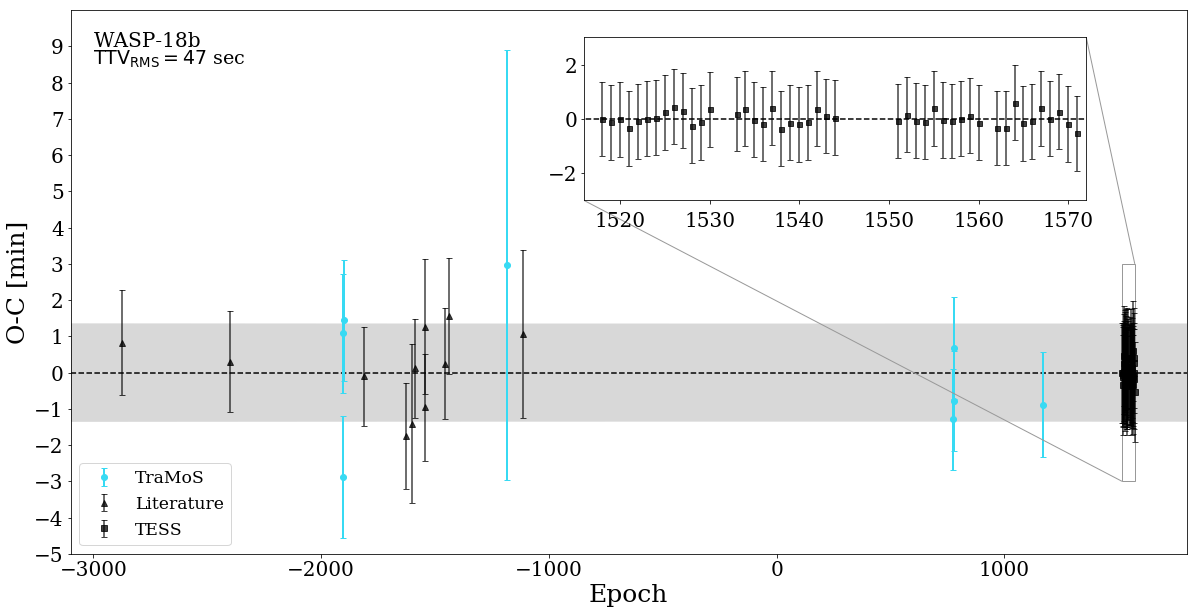
\includegraphics[width=1.0\textwidth]{imagenes/WASP18_TTV.png}
\caption{Observed minus calculated mid-transit times (TTV) for WASP-18b. The dashed black line corresponds to the proposed linear ephemeris, i.e. zero deviation from the predicted transit time  computed from our refined orbital period. For that, we considered 63 transit times from the TraMoS project (in light blue), published works and TESS (both in black). The grey area corresponds to the error propagation at $1\sigma$, where the quadratic trend looks almost horizontal.  The RMS scatter from the linear ephemeris is 47 seconds.}
\label{wasp18_ttv}
\end{figure*}

\subsubsection{WASP-19b}
%The best values of the parameters in Equation \ref{eq1} for WASP-19b are $T_{c}=2456402.7128^{+(17)}_{-(14)}\,[\rm{BJD_{TDB}}]$ and $P=0.78883852^{+(75)}_{-(82)}\,{\rm days}$. 

The proposed equation for linear ephemeris, considering 59 transit times of WASP-19b is:
\begin{equation} \label{eq1_w19}
T_{\rm C}(E)=2456402.7128\pm(16)+E \cdot 0.788838858\pm(47)
\end{equation}

The TTV values from the proposed linear ephemeris are listed in Table \ref{times_wasp19}, including transit times from the previous works \citep{Hebb2010,Anderson2010,Lendl2013,Tregloan2013,Bean2013,Mancini2013}. 

Figure~\ref{wasp19_ttv} shows the TTV values versus epoch, for all the transit time considered in this work.

The RMS from the linear ephemeris is about 75 seconds. The epoch of $-1011$ is the only one with a transit time deviation above $1.5\,\sigma$ from the linear ephemeris. If it is removed, then the RMS decreases to 69 seconds. Moreover, in our data the epoch $-611$ has one of the greatest errors due to bad weather conditions.

Considering all the transit times from Table~\ref{times_wasp19}, the linear fit has $\chi^{2}_{red} = 0.16$. This an indication of an overestimation of the errors. A second degree polynomial was also tested in order to reject or not a possible orbital decay. The goodness of that fit is $\chi^{2}_{red}=0.12$. 

\begin{longtable}{cccc}
\caption{Transit mid-times for WASP-19b}
\label{times_wasp19}
\tabularnewline
\hline \hline
Epoch & Transit mid-time & TTV & References\\
      & (${\rm BJD_{TDB}}$) & (min) &  \\
\hline
-2063 & $2454775.3372$ & $-1.6\pm3.2$ & 1\\
-2061 & $2454776.91566$ & $-0.5\pm2.3$ & 2 \\
-2010 & $2454817.14633$ & $-0.6\pm2.3$ & 3 \\
-1525 & $2455199.73343$ & $-0.2\pm2.6$& 4\\
-1459 & $2455251.79657$ & $-0.6\pm2.3$& 5 \\
-1458 & $2455252.58544$ & $-0.5\pm2.3$& 5 \\
-1454 & $2455255.74077$ & $-0.6\pm2.3$& 5 \\
-1449 & $2455259.68448$ & $-1.3\pm2.4$& 4 \\ 
-1431 & $2455273.88282$ & $-2.4\pm2.5$& 4 \\
-1399 & $2455299.12768$ & $0.6\pm2.4$& 4 \\
-1354 & $2455334.6254$ & $0.5\pm2.3$ & 6\\
-1349 & $2455338.56927$ & $0.1\pm2.3$& 3 \\ 
-1330 & $2455353.55659$ & $-0.8\pm2.3$& 6\\
-1317 & $2455363.81131$ & $-1.1\pm2.4$& 4  \\
-1311 & $2455368.54285$ & $-3.3\pm3.8$& 6 \\ 
-1094 & $2455539.72327$ & $0.2\pm2.4$ & 3 \\
-1056 & $2455569.69826$ & $-1.1\pm2.4$ & 3\\
-1039 & $2455583.10979$ & $0.8\pm2.6$ & 4 \\
-1037 & $2455584.68693$ & $0.0\pm2.3$ & 3 \\
-1025 & $2455594.15188$ &  $-1.6\pm3.3$ & 6 \\
-1016 & $2455601.25164$ & $-1.3\pm2.5$ & 6\\
-1014 & $2455602.83138$ & $1.7\pm2.4$ & 3 \\
-1011 & $2455605.19414$ & $-3.8\pm3.5$ & 6 \\
-1009 & $2455606.77464$ & $0.3\pm2.3$ & 3 \\
-1008 & $2455607.56241$ & $-1.2\pm2.4$ & 3 \\
-989 & $2455622.55057$ & $-0.9\pm2.3$ & 3 \\
-987 & $2455624.12787$ & $-1.5\pm3.1$ & 6 \\
-976 & $2455632.80612$ & $0.0\pm2.3$ & 3 \\
-947 & $2455655.68222$ & $-0.3\pm2.4$ & 3 \\
-928 & $2455670.66976$ & $-0.9\pm2.5$ & 3 \\
-923 & $2455674.61367$ & $-1.3\pm2.4$ & This work \\
-919 & $2455677.77038$ & $0.7\pm3.6$ & 6  \\
-905 & $2455688.81201$ & $-2.4\pm5.3$ & 6 \\
-904 & $2455689.60276$ & $0.4\pm2.4$ & 6 \\
-900 & $2455692.75674$ & $-1.6\pm4.3$ & 6 \\
-899 & $2455693.54639$ & $-0.5\pm2.3$ & 6  \\
-886 & $2455703.79933$ & $-3.3\pm6.4$ & 6 \\
-885 & $2455704.59078$ & $0.5\pm2.4$ & 6 \\
-880 & $2455708.534626$ & $0.0\pm 2.3$ & 6  \\
-654 & $2455886.81234$ &  $0.2\pm3.8$ & 6 \\
-642 & $2455896.27611$ & $-3.1\pm3.8$ & 6 \\
-618 & $2455915.20980$ & $-0.9\pm2.5$ & 6  \\
-613 & $2455919.15485$ & $0.4\pm 2.7$ & 6\\
-611 & $2455920.7353$ & $0.0\pm5.4$ & This work \\
-609 & $2455922.30966$ & $-0.4\pm8.3$ & 6 \\
-511 & $2455999.6163$ & $0.2\pm2.3$ & 7 \\
-483 & $2456021.70374$ & $0.1\pm2.3$ & 7 \\
-473 & $2456029.5925$ & $0.7\pm 2.4$ &3 \\
-468 & $2456033.53643$ &  $0.3\pm 2.3$ & 6  \\
-430 & $2456063.51174$ & $-0.5\pm 2.3$ & 3 \\
-86 & $2456334.87208$ & $-0.8\pm2.4$ & 4 \\
-47 & $2456365.6373$  & $-0.1\pm2.3$& This work \\
1 & $2456403.50158$ &  $-0.1\pm2.3$ & This work \\
729 & $2456977.77722$  & $1.3\pm2.3$ & 8 \\
867 & $2457086.63571$ & $-0.5\pm2.3$& This work \\
1383 & $2457493.67676$   & $-0.2\pm2.3$& This work  \\
1771 & $2457799.74612$ &  $-0.3\pm2.3$ & This work \\
1838 & $2457852.597807$ & $-0.7\pm2.3$ & This work\\ 
2064 & $2458030.8751$  & $-1.5\pm3.2$& This work \\
\hline
%\end{tabular}
%\tablebib{(1)~\citet{Hebb2010};
%(2) \citet{Anderson2010}; (3) \citet{Lendl2013}; (4) Exoplanet Transit Database (ETD) \url{var2.astro.cz/ETD}; (5) \citet{Tregloan2013}; (6) \citet{Mancini2013}; (7) \citet{Bean2013}; (8) \citet{Sedaghati2015}.}
\end{longtable} 

\begin{figure*}
%\vspace{0.1cm}\hspace{0.2cm}
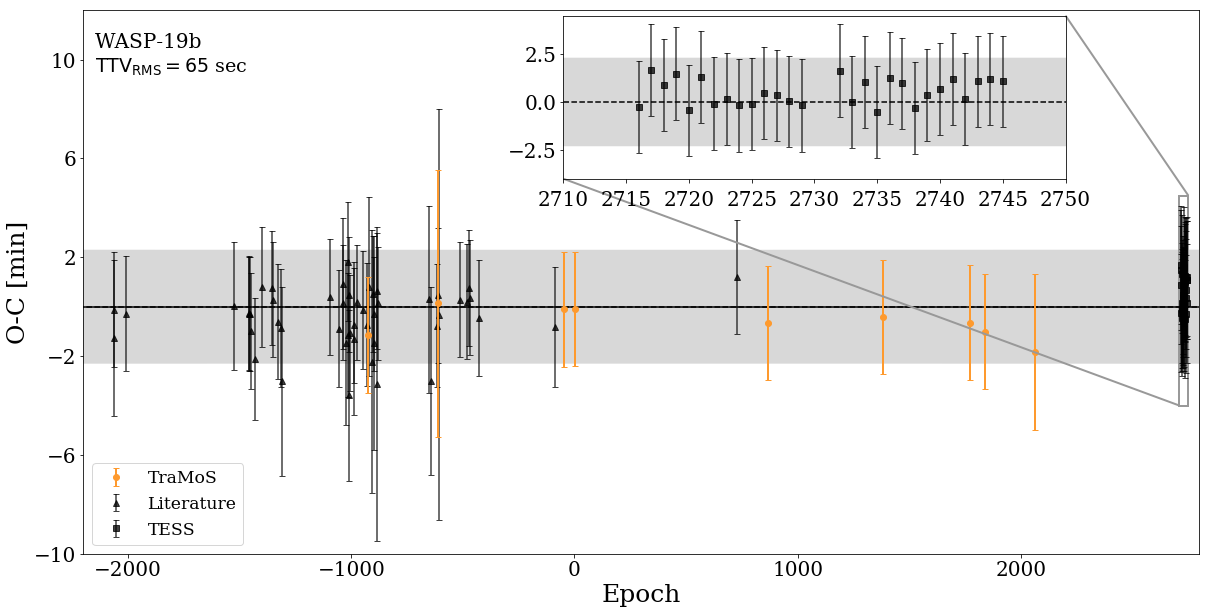
\includegraphics[width=1.0\textwidth]{imagenes/WASP19_TTV.png}
\caption{Observed minus calculated mid-transit times (TTV) for WASP-19b. The dashed black line corresponds to the proposed linear ephemeris, i.e. zero deviation from the predicted transit time  computed from our refined orbital period. For that, we considered 87 transit times from the TraMoS project (in light blue), published works and TESS (both in black). The grey area corresponds to the error propagation at $1\sigma$, where the quadratic trend looks almost horizontal.  The RMS scatter from the linear ephemeris is 65 seconds.}
\label{wasp19_ttv}
\end{figure*}

\subsubsection{WASP-77Ab}

As in the previous targets, we computed a refined linear ephemeris equation for WASP-77A considering 11 transit times:
\begin{equation} \label{eq1_w77}
T_{\rm C}(E)=2457420.88439\pm(85)+E \cdot 1.36002854\pm(52)
\end{equation}

In Table~\ref{tab:wasp77} are listed the TTV values of our transit times and from previous works \citep{Turner2016,Maxted2013} of WASP-77Ab and, at the bottom of Figure  XXX are plotted versus epoch. The scatter of all the transit times is about $RMS=121$ seconds. 

The epochs $175$ and $229$ are above $2\,\sigma$ from the expected transit time following the linear ephemeris, while all the others epochs lie within $1.5\,\sigma$ from it. When removing the epochs $175$ and $229$, the RMS decreases to 88 seconds. 

Considering all the transit times, the linear fit has $\chi^{2}_{red}=1.4$, and the second degree polynomial has $\chi^{2}_{red}=1.39$ . However, we chose the linear fit as it suppose a simpler model.

\begin{table}
\caption{Transit mid-times for WASP-77Ab}
\label{times_wasp77}
\centering
\begin{tabular}{cccc}
\hline \hline
Epoch & Transit mid-time & TTV & References\\
      & (${\rm BJD_{TDB}}$) & (min) &  \\
\hline
-1140 & $2455870.45054$ & $-2.0\pm1.5$ & 1 \\
-845 & $2456271.65888$ & $-2.0\pm1.4$ & 2 \\
-659 & $2456524.62617$ & $0.8\pm1.8$ & This work\footnote{a} \\
-606 & $2456596.70591$ & $-1.7\pm1.5$  & This work\footnote{a}  \\
-92 & $2457295.7626$  & $1.2\pm1.3$& This work \\
-89 & $2457299.84119$ &  $-1.0\pm1.3$ & This work \\
175 & $2457658.88744$ & $-2.8\pm1.5$ & This work\\
177 & $2457661.60987$   & $0.6\pm1.7$ & This work\footnote{a} \\
183 & $2457669.77054$ &  $1.4\pm1.4$  & This work  \\
229 & $2457732.33382$ & $4.2\pm1.4$& This work\footnote{a} \\
447 & $2458028.8159$  & $-1.8\pm6.5$ & This work\\ 
\hline
\end{tabular}
%\tablebib{(1) \citet{Maxted2013}; (2) \cite{Turner2016}.}
%\tablefoot{
%\tablefoottext{a}{From the Exoplanet Transit Database (ETD)  \url{var2.astro.cz/ETD}}}
\end{table}

\subsection{Limits on an Additional Perturber \label{addper}}
%Comments: Do not delete
%Written by Tobias C. Hinse
%The following text was largely taken from TEMPIV paper as the underlying methodology follows exactly that
%paper (and other papers).

The results from our mid-transit time study in Section~\ref{ttvsection}, allow us to infer an upper mass limit for an additional planet in each system. A perturbing planet will introduce a change in the mid-transit times of a known planet, which can be quantified by the RMS scatter around the nominal (unperturbed) linear ephemeris. The TTV effect is amplified for orbital configurations involving mean-motion resonances \citep{Agol2005, Holman2005, 2008ApJ...688..636N}. In principle, this amplification would allow the detection of a low-mass planetary perturbing body. A larger perturbation implies a larger RMS scatter around the nominal ephemeris.

The applied method follows the technique described in \citet{TEMP1,TEMP2,TEMP4}. The calculation of an upper mass limit is performed numerically via direct orbit integrations. For this task, we have modified the \texttt{FORTRAN}-based \texttt{MICROFARM}\footnote{\url{https://bitbucket.org/chdianthus/microfarm/src}}
package \citep{go2003,go2008} which utilizes OpenMPI\footnote{\url{https://www.open-mpi.org}} to spawn hundreds of single-task parallel jobs on a suitable super-computing facility. The package's main purpose is the numerical computation of the Mean Exponential Growth factor of Nearby Orbits
\citep[MEGNO]{cincsimo2000, go2001, ci2003} over a grid of initial values of orbital parameters for an $n$-body problem. The calculation of the RMS scatter of TTVs in the present work follows a direct brute-force method, which proved to be robust given the availability of computing power.

Within the framework of the three-body problem, we integrated the orbits of one of our three hot Jupiters and an additional perturbing planet around their host stars. The mid-transit time was calculated iteratively to a high precision from a series of back-and-forth integrations once a transit of the transiting planet was detected. The best-fit radii of both the planet and the host star were accounted for. We then calculated an analytic least-squares regression to the time-series of transit numbers and mid-transit times to determine a best-fitting linear ephemeris with an associated RMS statistic for the TTVs. The RMS statistic was based on a 20-year integration corresponding to 7763 transits for WASP-18b, 9270 transits for WASP-19b, and 5371 transit events for WASP-77Ab. This procedure was then applied to a grid of masses and semi-major axes of the perturbing planet while fixing all the other orbital parameters. In this study, we have chosen to start the perturbing planet on a circular orbit that is co-planar with the transiting planet; this implies that $\Omega_2=0^{\circ}$ and $\omega_2=0^{\circ}$ for the perturbing and $\Omega_1 = 0^{\circ}$ for the transiting planet. This setting provides a most conservative estimate of the upper mass limit of a possible perturber \citep{bean2009, fukui2011, Hoyer2011, Hoyer2012}. For the interested readers, we refer to \citet{TEMP4}, which has studied the effects of TTVs on varying initial orbital parameters.

\begin{table}
\caption{Approximate upper mass limits of a putative perturber in various orbital resonances for each system}
\label{masstable}
\centering
\begin{tabular}{cccc}
\hline \hline
MMR & WASP-18 & WASP-19 & WASP-77A \\
($P_{2}/P_{1}$) & $[M_{\oplus}]$ & $[M_{\oplus}]$ & $[M_{\oplus}]$ \\
\hline
1:3 & 1.9    & 500\footnote{b} & 1.0 \\
2:5 & 4.0    & -   & -   \\
1:2 & 5.0\footnote{a} & 2.0 & 3.5 \\
3:5 & -      & -      & 2.0 \\
2:3 & -      & -      & 7.0\footnote{a} \\
5:3 & -      & 6.0    & 6.0   \\
7:4 & -      & -      & 10.0 \\
2:1 & 25\footnote{a}    & 0.9    & 3.5 \\
7:3 & 80.0\footnote{c}   & -      & -   \\
5:2 & 10.0   & 3.0    & -   \\
3:1 & 7.0    & 2.0    & 4.5 \\
17:5 & 500.0\footnote{d} & -      & -    \\
4:1 & 50.0   & 100.0\footnote{e}  & 60.0\footnote{f} \\
\hline
\end{tabular}
%\tablefoot{
%\tablefoottext{a}{Very close to the general instability area.}
%\tablefoottext{b}{This value is constraint by RV limit of 17.8 $[M_{\oplus}]$}
%\tablefoottext{c}{This value is constraint by RV limit of 74.6 $[M_{\oplus}]$}
%\tablefoottext{d}{This value is constraint by RV limit of 82.8 $[M_{\oplus}]$}
%\tablefoottext{e}{This value is constraint by RV limit of 40.8 $[M_{\oplus}]$}
%\tablefoottext{f}{This value is constraint by RV limit of 30.8 $[M_{\oplus}]$}}
\end{table} 

In order to calculate the location of mean-motion resonances, we have used the same code to calculate MEGNO on the same parameter grid. However, this time we integrated each initial grid point for 1000 years, allowing this study to highlight the location of weak chaotic high-order mean-motion resonances. In short, MEGNO quantitatively measures the degree of stochastic behaviour of a non-linear dynamical system and has been proven useful in the detection of chaotic resonances \citep{go2001, hi2010}. In addition to the Newtonian equations of motion, the associated variational equations of motion are solved simultaneously allowing the calculation of MEGNO at each integration time step. The \texttt{MICROFARM} package implements the \texttt{ODEX}\footnote{\url{https://www.unige.ch/~hairer/prog/nonstiff/odex.f}} extrapolation algorithm to numerically solve the system of first-order differential equations.

Following the definition of MEGNO \citep{cincsimo2000} (denoted as $\langle Y\rangle$ in Figures~\ref{megno_wasp18}-\ref{megno_wasp77}), in a dynamical system that evolves quasi-periodically, the quantity $\langle Y \rangle$ will asymptotically approach 2.0 for $t \rightarrow \infty$. In that case, often the orbital elements associated with that orbit are bounded. In case of a chaotic time evolution, the $\langle Y\rangle$ diverges away from 2.0 with orbital parameters exhibiting erratic temporal excursions. For quasi-periodic orbits, we typically have $|\langle Y \rangle - 2.0| < 0.001$ at the end of each integration.

Importantly, MEGNO is unable to prove that a dynamical system is evolving quasi-periodically, meaning that a given system cannot be proven to be stable or bounded for all times. The integration of the equations of motion only considers a limited time period. However, once a given initial condition has found to be chaotic, there is no doubt about its erratic nature in the future.

In the following, we will present the results of each system for which we have calculated the RMS scatter of TTVs on a grid of the masses and semi-major axes of a perturbing planet in a circular, co-planar orbit. Results are shown in Figures~\ref{megno_wasp18} - \ref{megno_wasp77} and Table \ref{masstable}. In each of the three cases, we find the usual instability region located in the proximity of the transiting planet with MEGNO color-coded as yellow (corresponding to $\langle Y\rangle > 5$). The extent of these regions coincides with the results presented in \citet{barnes2006}. The locations of mean-motion resonances are indicated by arrows in each map.


\subsubsection{WASP-18b}
For the WASP-18b system we find a large region of instability when
compared to the other two systems with the boundaries at the 1:2 interior
and 2:1 exterior mean-motion resonance. By over-plotting the RMS scatter
of mid-transit times ($\rm TTV_{\rm RMS}$) for a certain value, we find
that the TTVs are relatively more sensitive at orbital architectures
involving mean-motion resonances confirming the results by
\citet{Agol2005} and \citet{Holman2005}. This also applies to WASP-19 and
WASP-77A.

As shown in Figure~\ref{megno_wasp18}, we find that a perturbing body of mass (upper limit) around $7-500~M_{\oplus}$ will produce an RMS of $83\,{\rm s}$ when located in the $P_2/P_1=$ 7:3, 5:2, 3:1, 17:5 and 4:1 exterior resonance. For the 1:3 interior resonance, a perturber mass (upper limit) as small as $1.9~M_{\oplus}$ could also cause a RMS mid-transit time scatter of $83\,{\rm s}$.

\subsubsection{WASP-19b}
For the WASP-19b system the measured transit-timing RMS scatter was $\rm TTV_{\rm RMS}=75,\rm s$. Additional bodies with a mass of $500~M_{\oplus}$ and as low as $2.0~M_{\oplus}$ and $0.9~M_{\oplus}$ at the 1:3, 1:2 (interior) and 2:1 (exterior) mean-motion resonances could cause the observed RMS scatter. Hypothetical planets of $6~M_{\oplus}$, $3~M_{\oplus}$ and $2~M_{\oplus}$ could cause the observed RMS scatter at the 5:3, 5:2 and 3:1 exterior mean-motion resonances, respectively. We refer to Fig.~\ref{megno_wasp19}.

\subsubsection{WASP-77Ab}
For the WASP-77Ab system the results are somewhat similar to WASP-19b. We refer to Fig.~\ref{megno_wasp77}. The measured RMS of mid-transit timing variations around the linear ephemeris was $\rm TTV_{\rm RMS}=121\rm s$. For interior mean-motion resonances the 1:2 and 2:3 commensurabilities could cause the observed $\rm TTV_{\rm RMS}$ by an additional planet of mass around $3.5~M_{\oplus}$ and $7~M_{\oplus}$. However, the 2:3 resonance is very close to the general instability area rendering the orbit likely to be unstable. Further a $1~M_{\oplus}$ mass planet at the 1:3 interior resonance could also cause a $\rm TTV_{\rm RMS}$ of 121 s. A $2~M_{\oplus}$ mass planet located at the 3:5 resonance, although relatively close to the inner edge of the general instability region, could also explain the observed timing variation. For exterior 
mean-motion resonances of 2:1, 3:1 and 4:1 an additional planet of mass $3.5~M_{\oplus}, 4.5~M_{\oplus}$ and $60~M_{\oplus}$, could cause a $\rm TTV_{\rm RMS}=121\rm s$, respectively. A subtle difference from the WASP-19b system is found at the 5:2 resonance, which does not exhibit any significant decrease in upper mass planet detection sensitivity.

\subsection{TTV period search}

We have carried out a Lomb-Scargle period analysis \citep{Lomb1976, Scargle1982} for each system's TTVs residuals to search for a significant periodic trend. For this we applied the \texttt{LombScargle}\footnote{\url{http://docs.astropy.org/en/stable/stats/lombscargle.html}} (LS) algorithm available within the \texttt{Astropy} (v3.1.1) Python package \citep{2012cidu.conf...47V, 2015ApJ...812...18V}.

The algorithm is suitable for unevenly-sampled data. We chose to carry out computations using the observed transit epochs for each system as the independent variable. Each epoch is determined with a high degree of confidence. TTV measurement uncertainties were not accounted for since no convincing periodic trend were detected. Default settings were avoided in order to safeguard the analysis from an inappropriate frequency grid choice. We made use of the minimum and maximum frequency heuristic. Periods between 1 and 5000 epochs were searched for. Furthermore, we sampled each peak twelve times. Noteworthy to mention, and often overlooked, is the possible detection of frequencies much larger than the Nyquist sampling frequency \citep{2018ApJS..236...16V}. 

The result for each system is shown in Figs.~\ref{LS_wasp18_random} to \ref{LS_wasp77_random}, were we show the Lomb-Scargle power $P$ from the standard normalization method with $0\le P<1$. The final period is found by multiplying with the final best-fit period for each system. To quantify the significance of period-peaks we calculated the false-alarm probability (FAP) for three different $p$-values. The FAP encodes the probability of detecting a peak of a given height (or higher) and is conditioned on the null-hypothesis that the data is characterized by normal random noise. 

To avoid misinterpretation of the FAP we have calculated synthetic random TTVs for each system in a single realization. For each known epoch, we drew a normal random point with mean zero and standard deviation in accordance with the measured RMS for each timing data set (83 s for WASP-18, 75 s for WASP-19 and 121 s for WASP-77A).

We then recomputed the LS periodogram for each synthetic data set. This method enables a meaningful quantitative assessment of a minimum requirement of the FAP to detect a true periodic signal which clearly stands out from Gaussian noise. We plot the LS periodograms for the synthetic TTVs in the bottom panels of Figs.~\ref{LS_wasp18_random} to \ref{LS_wasp77_random}. For the case of WASP-19 and WASP-77, we found that a reasonable minimum FAP of 0.01\% is required in order to distinguish any signal from white noise. For the case of WASP-18 the threshold is just above 0.01\%. In generally, we found no significant (99.99\% level) periodicity peaks for all three cases.
%However, with some good will, qualitatively, the LS periodogram for WASP-19 shows a slight decrease in FAP for two periods (at 0.8 and 1.2 in Fig. \ref{LS_wasp19_random}) when compared to the white noise data case.

\begin{figure}
%% Toby's internal figure note (DO NOT DELETE!!):
%% Project path: /home/tobiash/simulations/TRAMOS_PiaCortesZuleta/TTVMEGNOMAPS/WASP18
%% imported to GIMP, resolution 300, anti-aliasing, rotated, cropped (removing white space), added alpha 
%% channel, scaled to 12cm, then saved as PNG
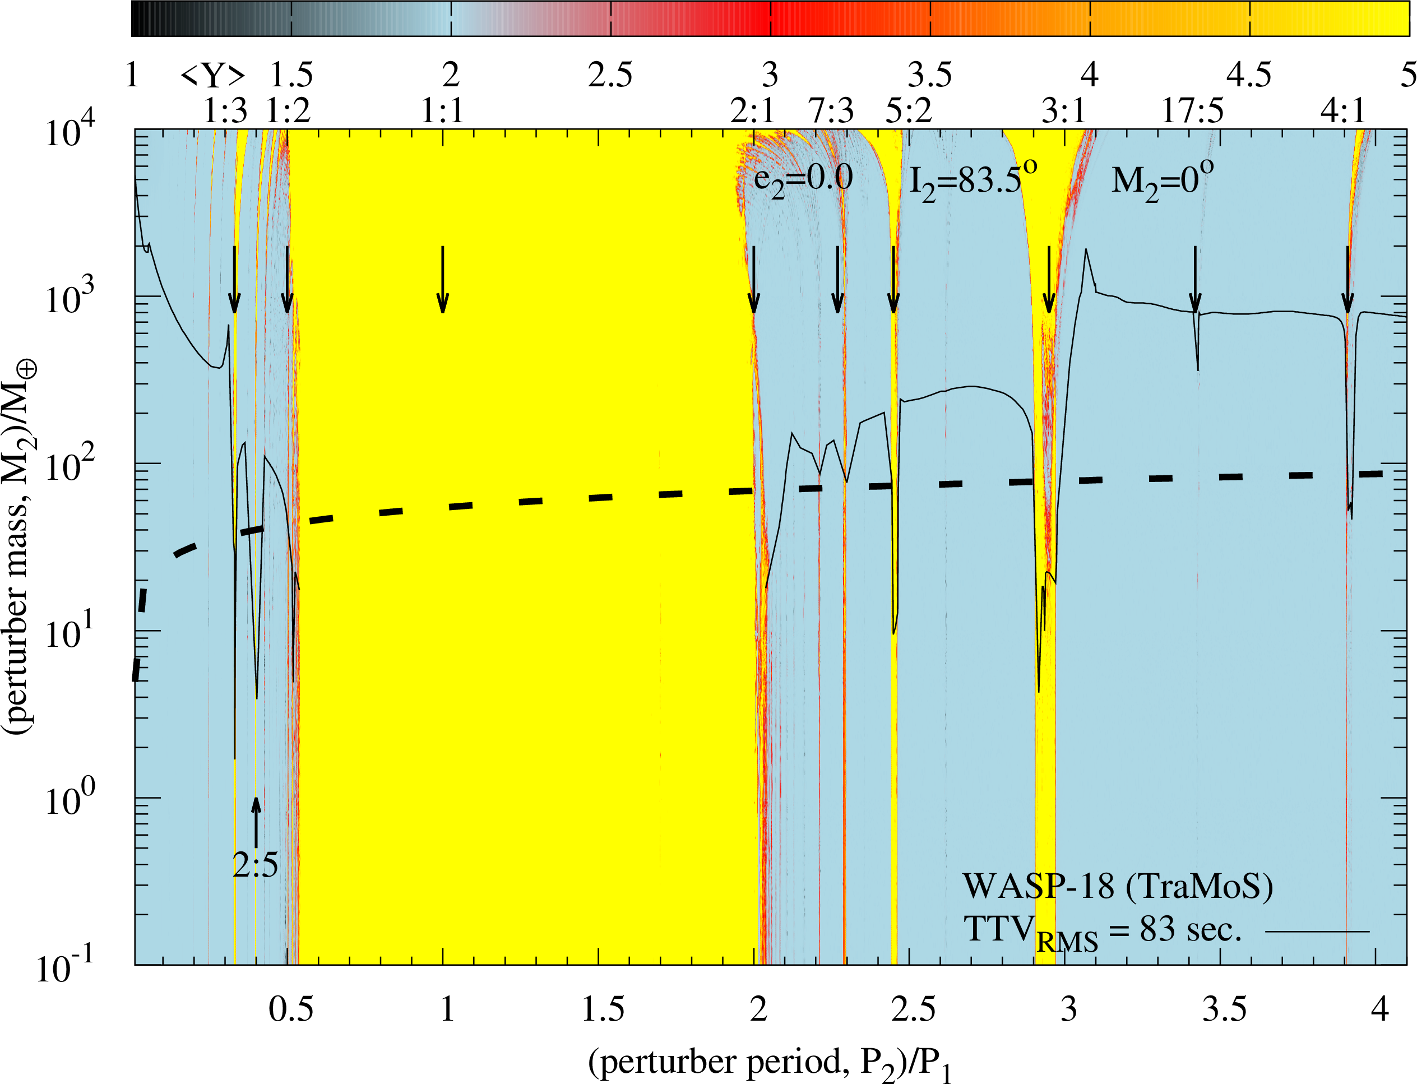
\includegraphics[width=1.0\columnwidth]{imagenes/WASP18_TraMos_83sec_Map001_GIMP_scaled.png}
\caption{MEGNO ($\langle Y \rangle$) stability map for the WASP-18 system. We over-plot the map with an upper mass of a hypothetical perturbing planet introducing a mid-transit time $\rm TTV_{\rm RMS}$ scatter of $83\,{\rm s}$ (solid line) as obtained in this study. The stipulated line is the upper mass limit as obtained from the RMS scatter $(30.9\, \rm m/s)$ of the radial-velocity curve. For initial conditions resulting in a quasi-periodic (i.e bounded) motion of the system, the $\langle Y\rangle$ value is close to 2.0 (color coded blue). For chaotic (i.e unstable) motion, the $\langle Y \rangle$ is diverging away from 2.0 (color coded red to yellow). Vertical arrows indicate $(P_2/P_1)$ orbital resonances between the perturbing body and the transiting planet. The two planets were assumed to be co-planar, and the perturbing planet's eccentricity was initially set to zero.
\emph{See electronic version for colors}.}
\label{megno_wasp18}
\end{figure}

\begin{figure}
%% Toby's internal figure note (DO NOT DELETE!!):
%% Project path: /home/tobiash/simulations/TRAMOS_PiaCortesZuleta/TTVMEGNOMAPS/WASP19
%% imported to GIMP, resolution 300, anti-aliasing, rotated, cropped (removing white space), added alpha 
%% channel, scaled to 12cm, then saved as PNG
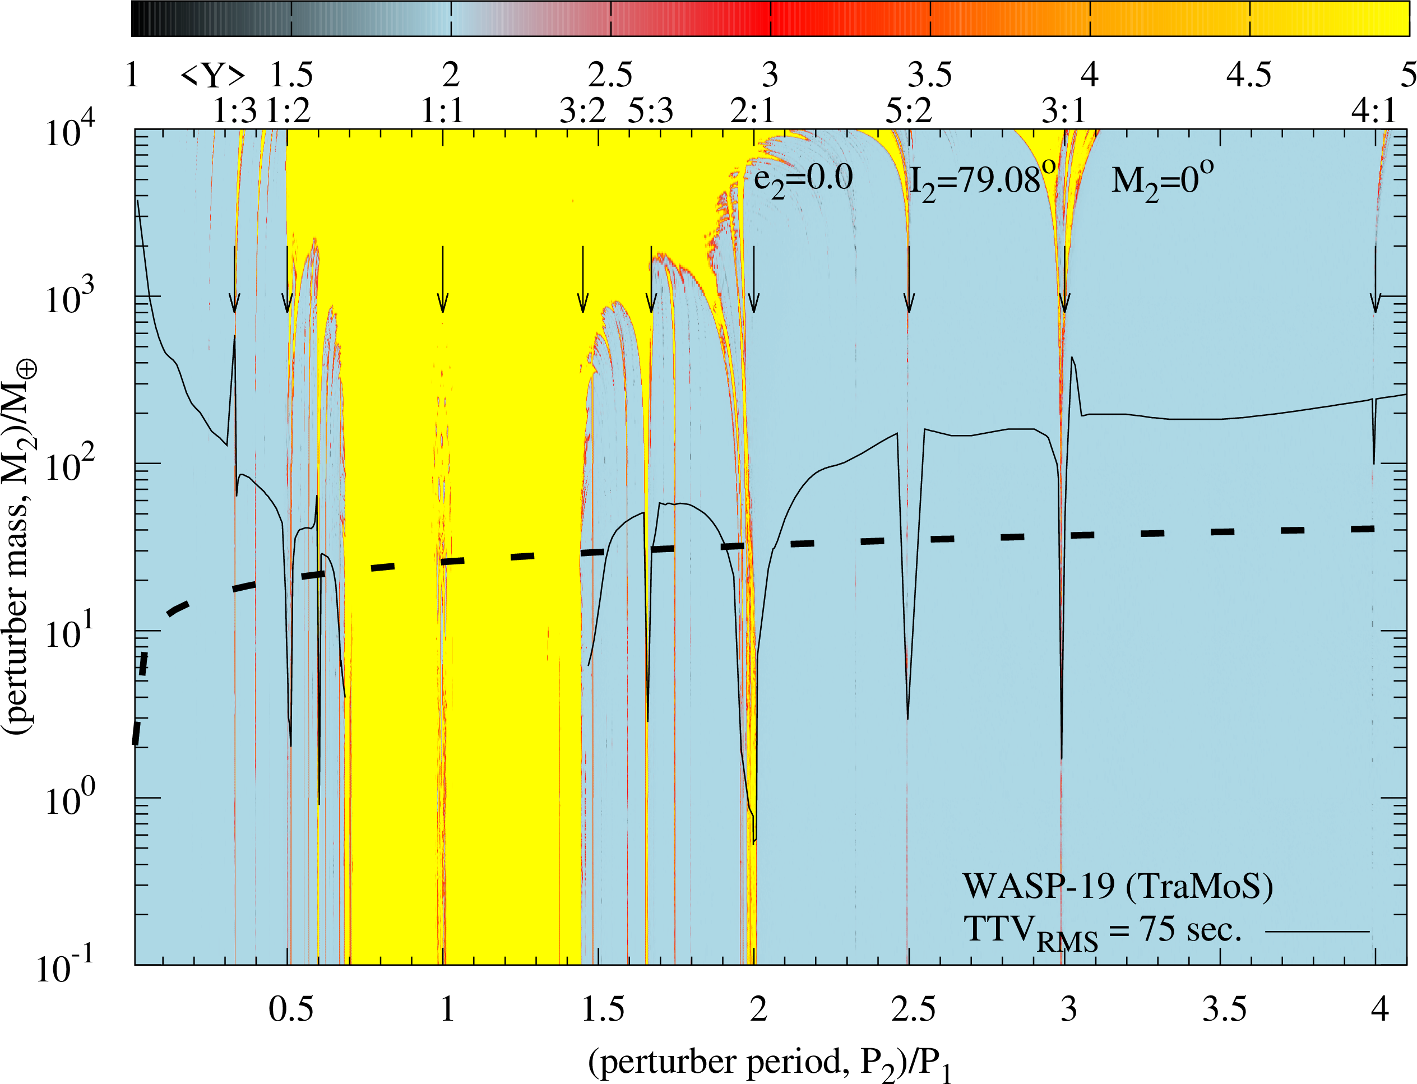
\includegraphics[width=1.0\columnwidth]{imagenes/WASP19_TraMos_Map001_GIMP_scaled.png}
\caption{Same as Fig.~\ref{megno_wasp18}, but this time for WASP-19 with an $\rm TTV_{\rm RMS}$ of 75 s. The
RMS for the radial-velocity measurements was $(18.2\,\rm m/s)$. \emph{See electronic version for colors}.}
\label{megno_wasp19}
\end{figure}

\begin{figure}
%% Toby's internal figure note (DO NOT DELETE!!):
%% Project path: /home/tobiash/simulations/TRAMOS_PiaCortesZuleta/TTVMEGNOMAPS/WASP77
%% imported to GIMP, resolution 300, anti-aliasing, rotated, cropped (removing white space), added alpha 
%% channel, scaled to 12cm, then saved as PNG
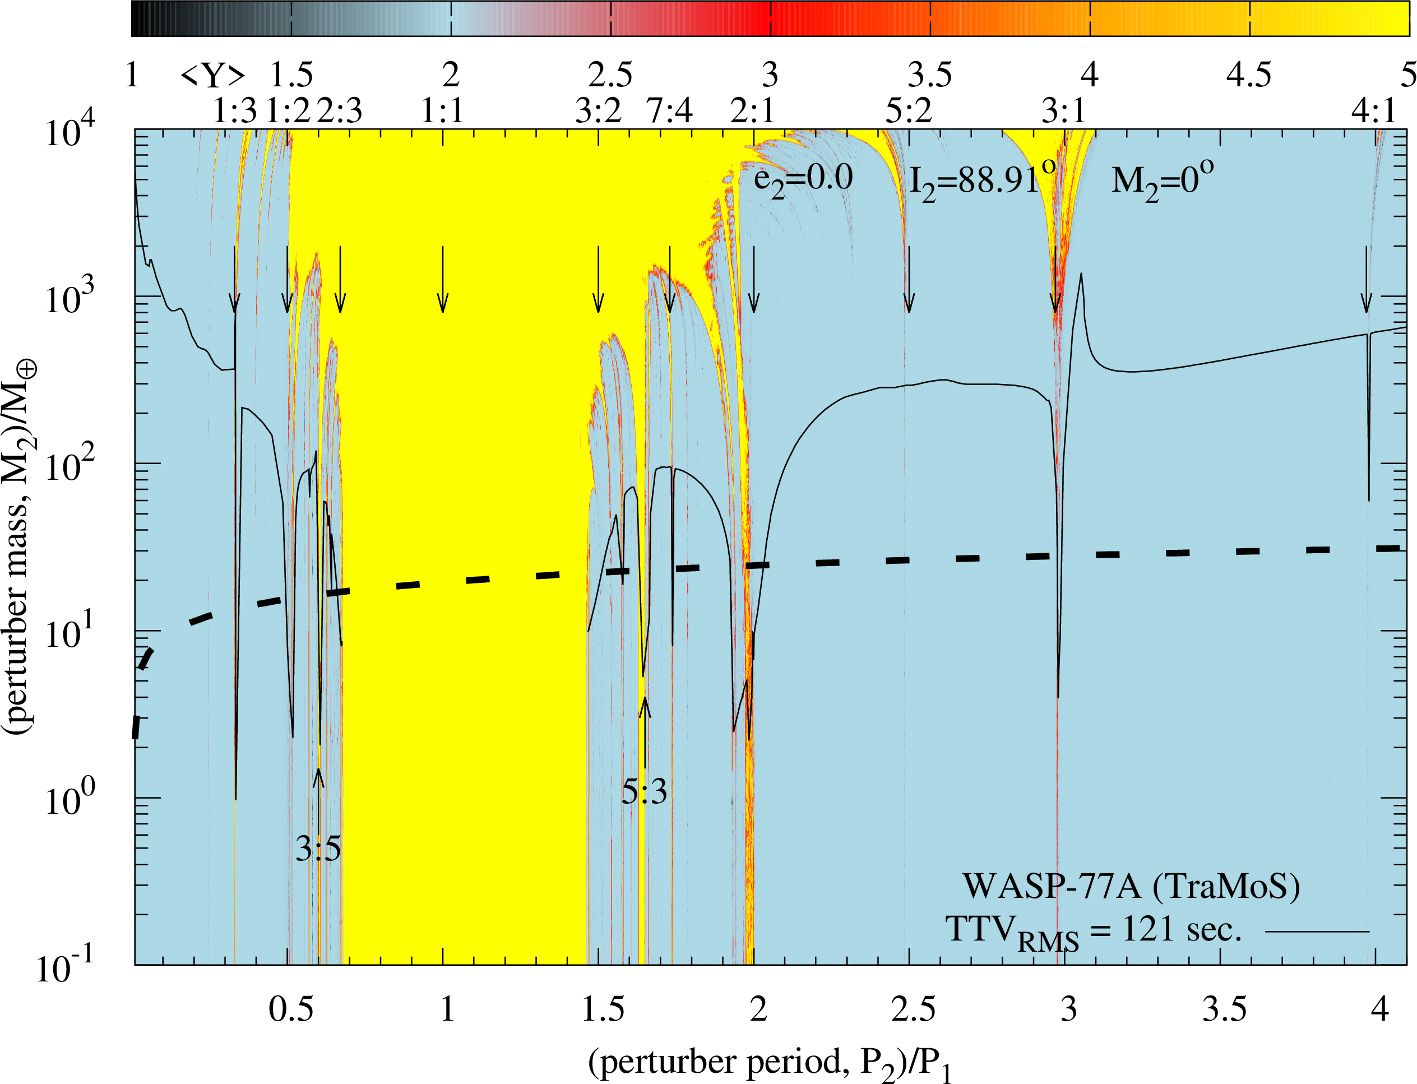
\includegraphics[width=1.0\columnwidth]{imagenes/WASP77_TraMos_121sec_Map001_GIMP_scaled.png}
\caption{Same as Fig.~\ref{megno_wasp18}, but this time for WASP-77 with an $\rm TTV_{\rm RMS}$ of 121 s. The RMS for the radial-velocity measurements was $(12.0\,\rm m/s)$.
\emph{See electronic version for colors}.}
\label{megno_wasp77}
\end{figure}

\begin{figure*}
\centering
%% Toby's internal figure note (DO NOT DELETE!!):
%% Project path: /home/tobiash/simulations/TRAMOS_PiaCortesZuleta/LombScargle/GnuPlotPlotting/WASP18
%% Project path: /home/tobiash/simulations/TRAMOS_PiaCortesZuleta/LombScargle/Python/WASP18/testingLS
%% GIMP, original was rotated, cropped (removing white space), scaled to 120cm, then saved as PNG
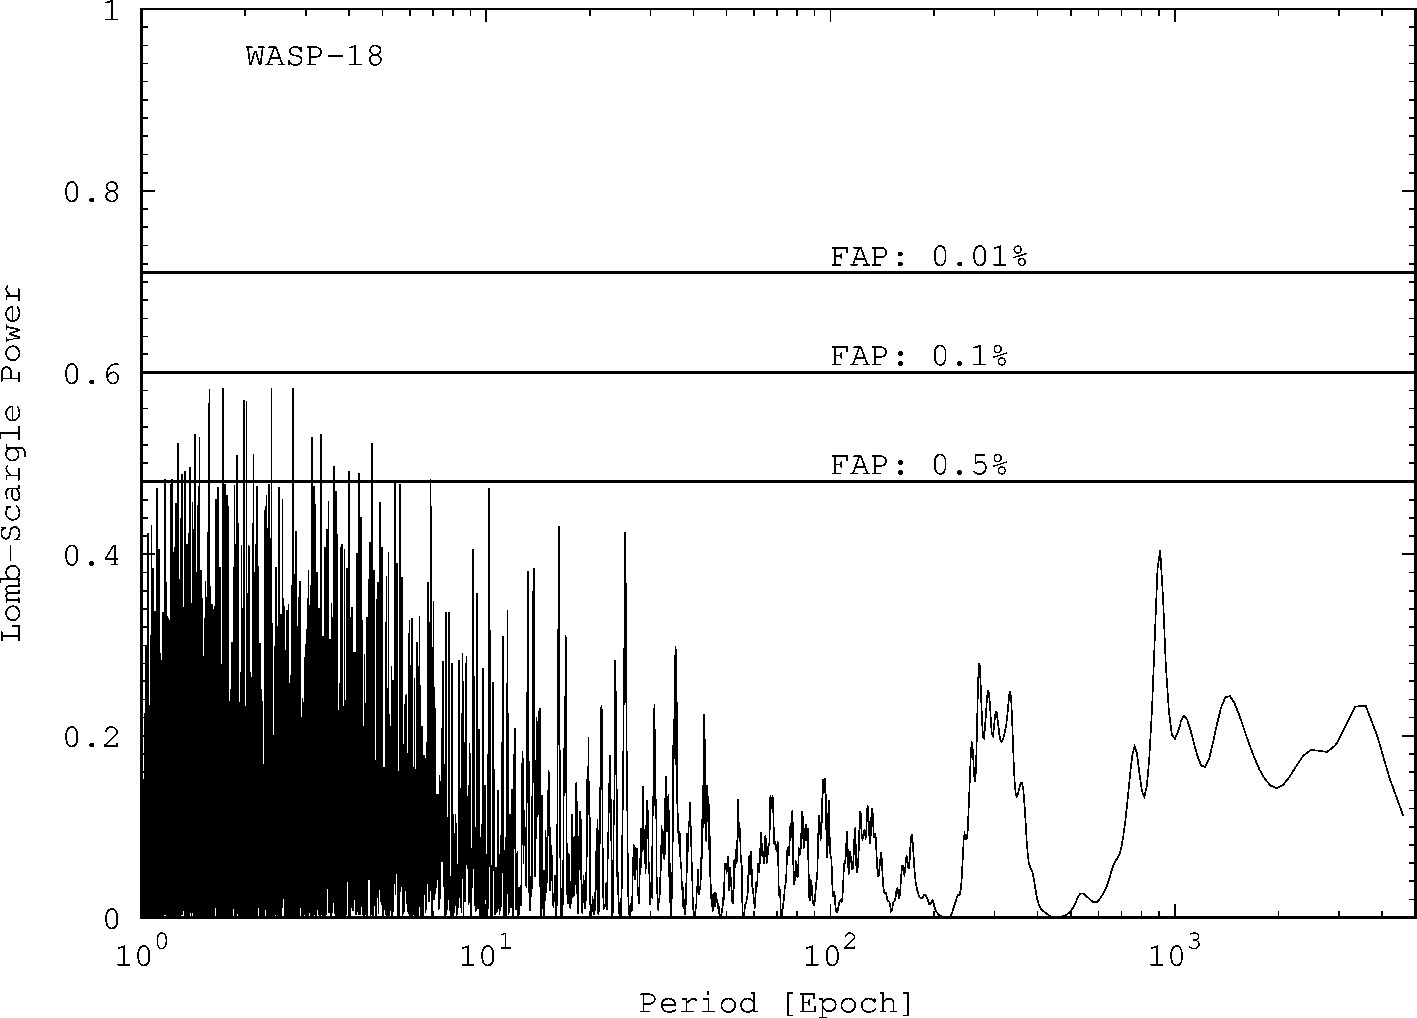
\includegraphics[width=0.7\columnwidth]{imagenes/LS_WASP18_New_GIMP.png}
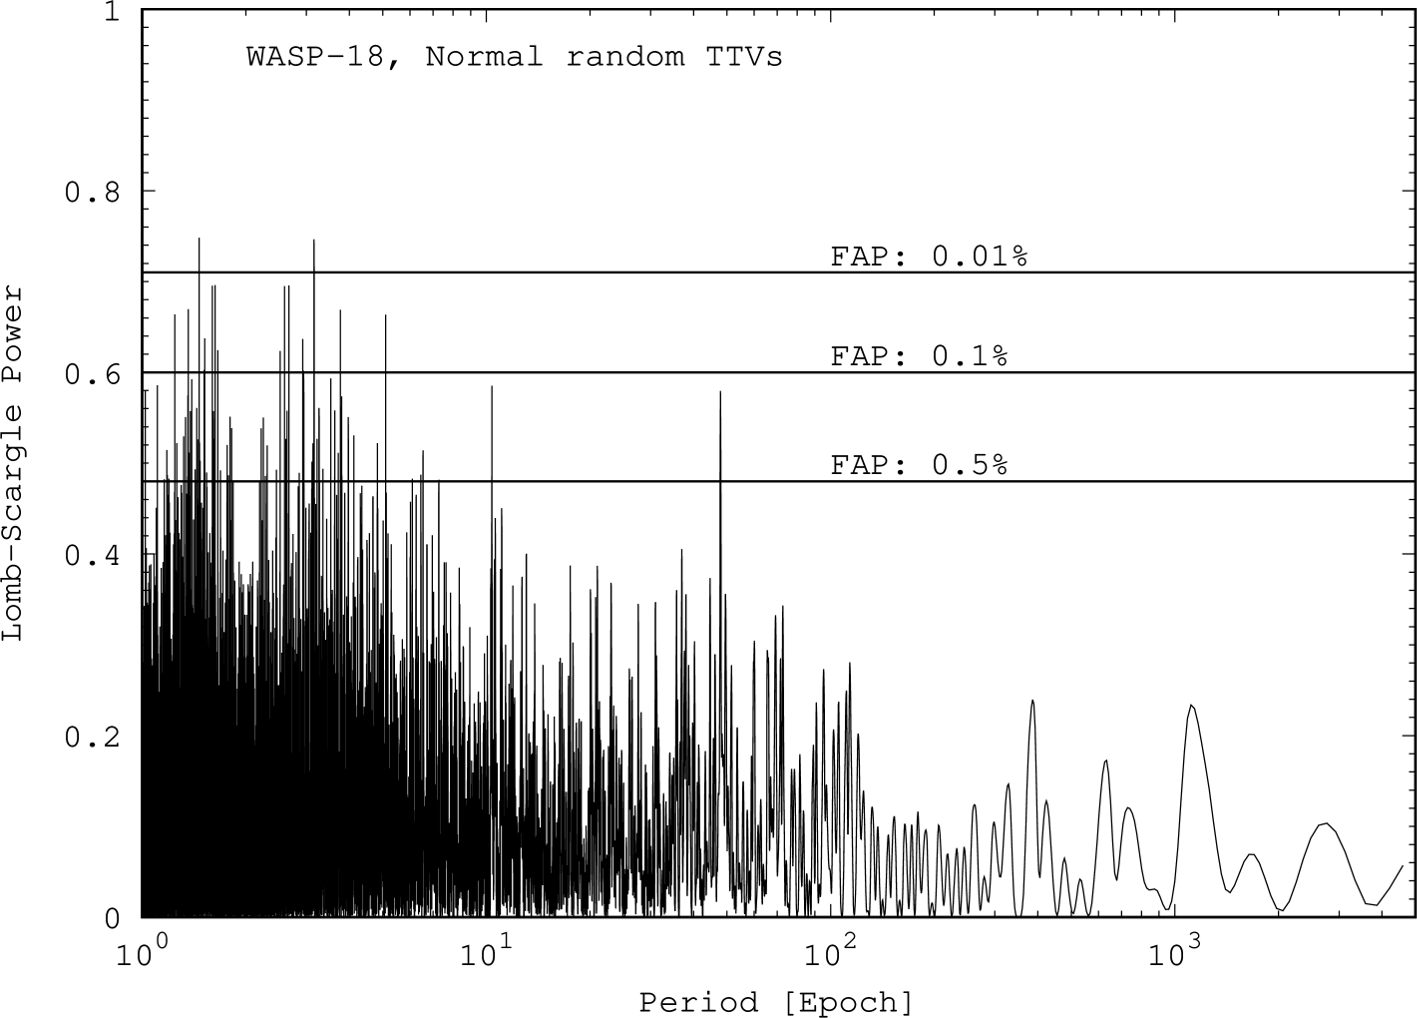
\includegraphics[width=0.7\columnwidth]{imagenes/LS_WASP18_NormRandom_New_GIMP.png}
\caption{Lomb-Scargle (standard normalized) power vs period for observed TTV residuals of WASP-18 (\emph{top panel}) and for a simulated set of TTVs randomly drawn from a normal distribution with mean zero and standard deviation of 1.38 minutes (\emph{lower panel}). See text for more details.}
\label{LS_wasp18_random}
\end{figure*}

\begin{figure*}
\centering
%% Toby's internal figure note (DO NOT DELETE!!):
%% Project path: /home/tobiash/simulations/TRAMOS_PiaCortesZuleta/LombScargle/GnuPlotPlotting/WASP19
%% Project path: /home/tobiash/simulations/TRAMOS_PiaCortesZuleta/LombScargle/Python/WASP19/testingLS
%% GIMP, original was rotated, cropped (removing white space), scaled to 120cm, then saved as PNG
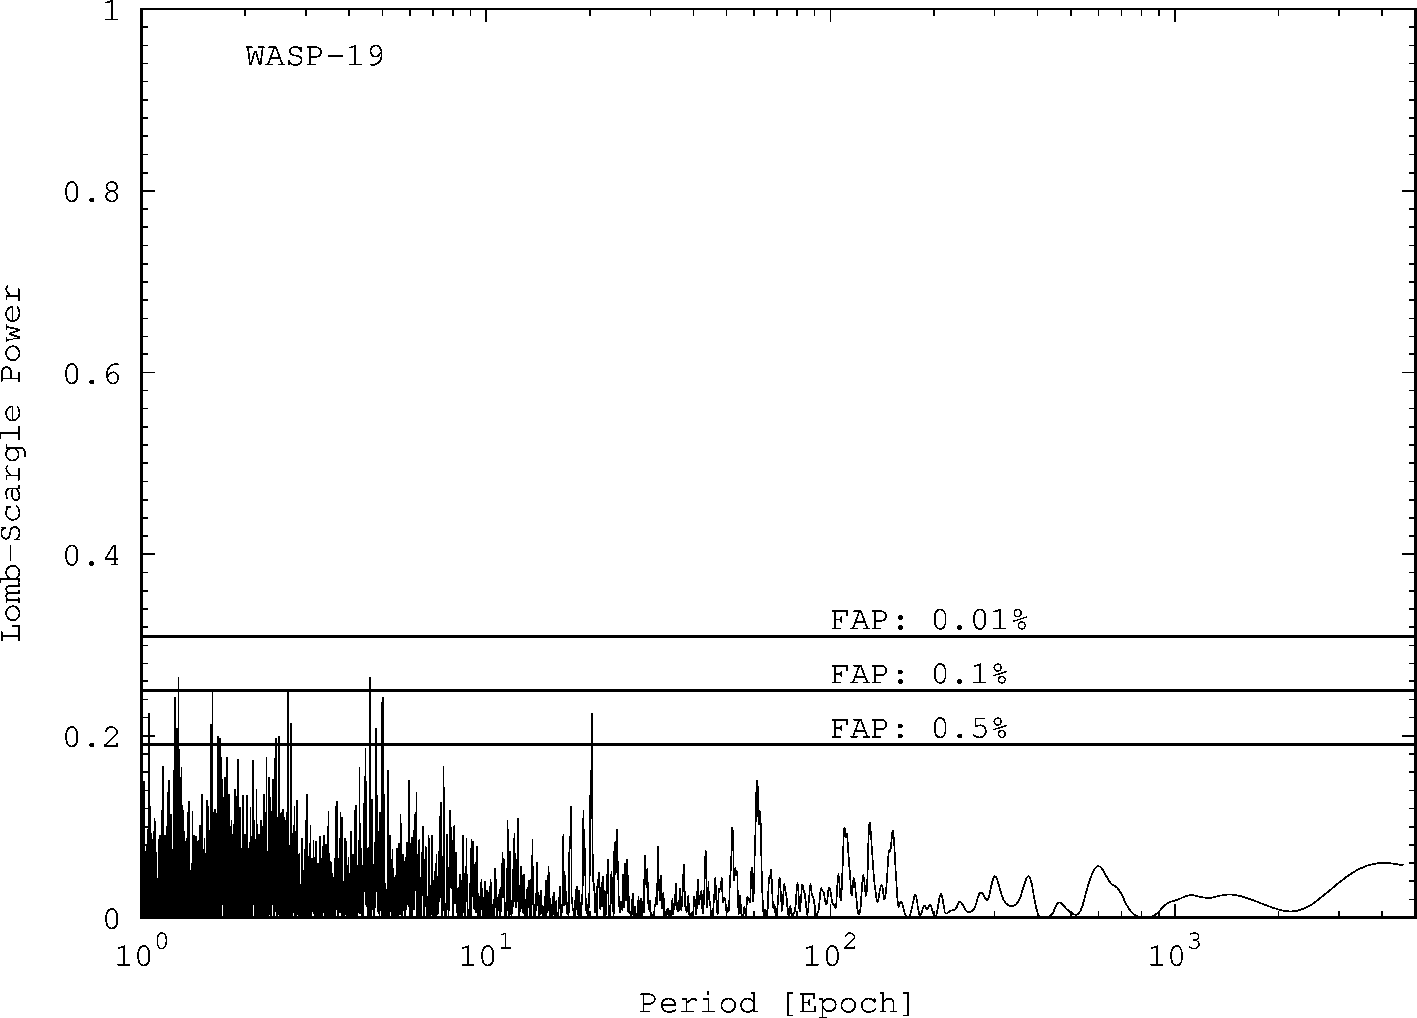
\includegraphics[width=0.7\columnwidth]{imagenes/LS_WASP19_New_GIMP.png}
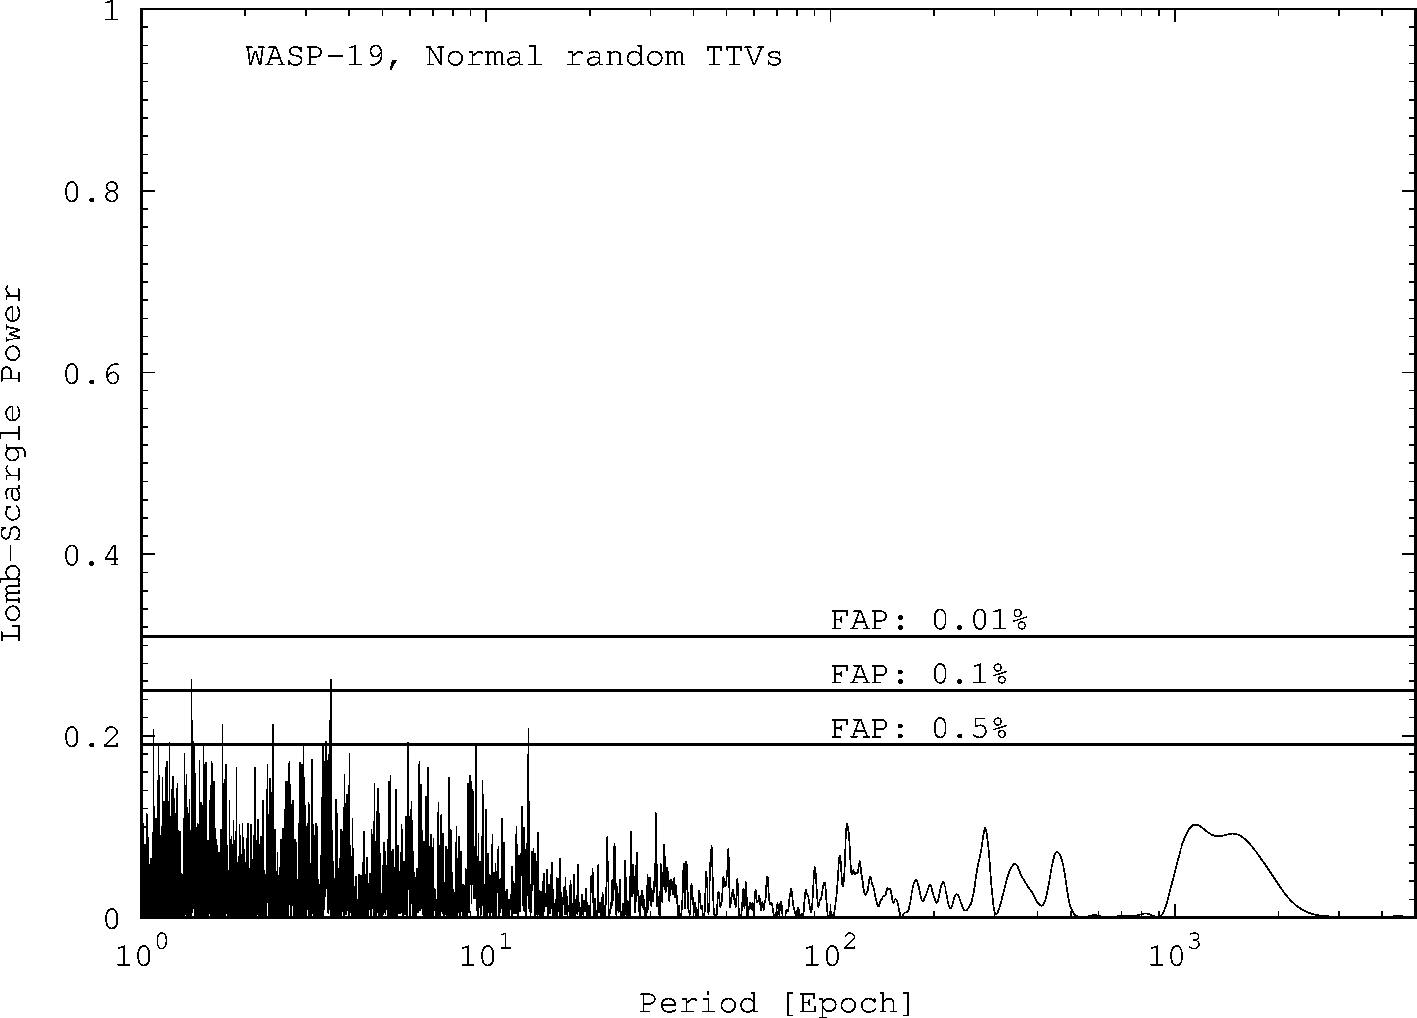
\includegraphics[width=0.7\columnwidth]{imagenes/LS_WASP19_NormRandom_New_GIMP.png}
\caption{Lomb-Scargle (standard normalized) power vs period for observed TTV residuals of WASP-19 (\emph{top
panel}) and for a simulated set of TTVs randomly drawn from a normal distribution with mean zero and standard
deviation of 1.33 minutes (\emph{lower panel}). See text for more details.}
\label{LS_wasp19_random}
\end{figure*}

\begin{figure*}
\centering
%% Toby's internal figure note (DO NOT DELETE!!):
%% Project path: /home/tobiash/simulations/TRAMOS_PiaCortesZuleta/LombScargle/GnuPlotPlotting/WASP77
%% Project path: /home/tobiash/simulations/TRAMOS_PiaCortesZuleta/LombScargle/Python/WASP77/testingLS
%% GIMP, original was rotated, cropped (removing white space), scaled to 120cm, then saved as PNG
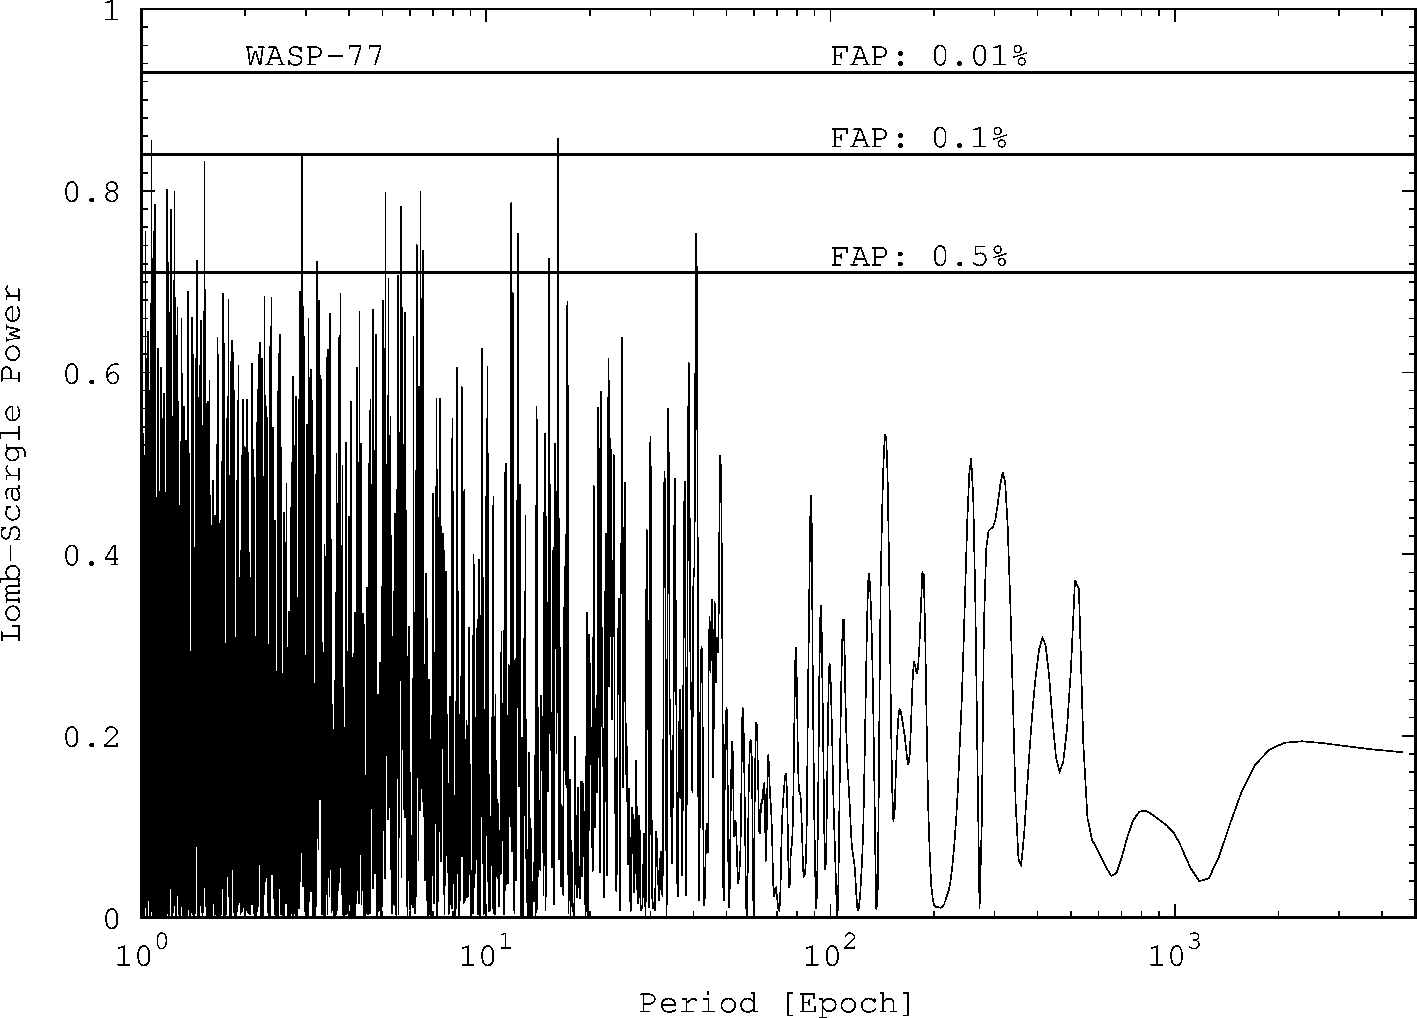
\includegraphics[width=0.7\columnwidth]{imagenes/LS_WASP77_New_GIMP.png}
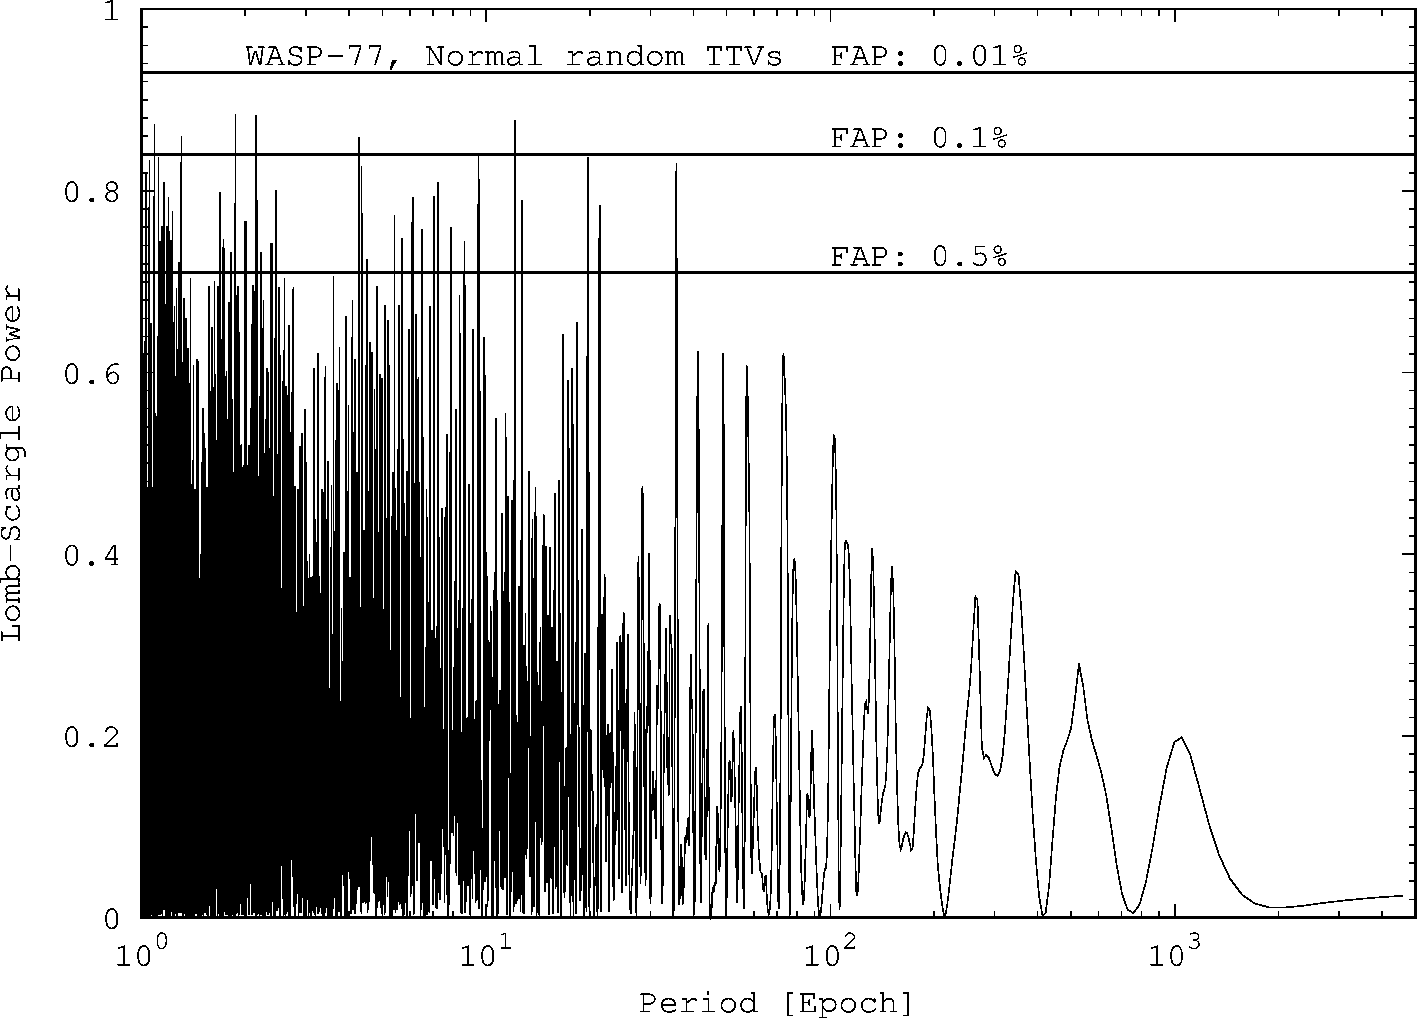
\includegraphics[width=0.7\columnwidth]{imagenes/LS_WASP77_NormRandom_New_GIMP.png}
\caption{Lomb-Scargle (standard normalized) power vs period for observed TTV residuals of WASP-77 
(\emph{top panel}) and for a simulated set of TTVs randomly drawn from a normal distribution with mean zero
and standard deviation of 2.02 minutes (\emph{lower panel}). See text for more details.}
\label{LS_wasp77_random}
\end{figure*}

\section{Summary and Conclusions}\label{summary}
We performed photometric follow-ups of the transiting exoplanets WASP-18b, WASP-19b and WASP-77Ab with one meter-class telescopes within the TraMoS project. Our 22 new high-precision light curves and archive data were combined together to refine physical and orbital parameters of the systems. 

For WASP-18b we find a larger value for the fraction of the radius $R_p/R_*$ than the most recent work with TESS data \cite{Shporer2018}, and a larger total transit duration $T_{14}$ comparing with \cite{Hellier2009}. The rest of stellar and planetary parameters are all in good agreement with previous results.

In the analysis of WASP-19b, our results are in general, in good agreement with previous works \citep{Hebb2010,Lendl2013}. Only the inclination $i$ and the total duration of the transit $T_{14}$ show important differences. 

In this work we reported the first bulk measurements of the WASP-77Ab system. We find almost no disagreement in the orbital and physical parameters with the discovery paper \cite{Maxted2013}.

We included archival transit times along with the transits from the TraMoS project to obtained refined values for the period $P$ of the three exoplanets, as well as updated linear ephemeris. We report a period of $P=0.94145223\pm9\times10^{-8}$ days for WASP-18b, $P=0.788838852\pm5\times10^{-9}$ days for WASP-19b, and $P=1.3600285\pm5\times10^{-7}$ days for WASP-77Ab. With the proposed linear ephemeris we found $\rm TTV_{RMS}$ of 83 seconds, 75 seconds, and 121 seconds, for WASP-18b, WASP-19b, and WASP-77Ab, respectively. Also, we find a lack of significant TTV periodic signals.  

The $\rm TTV_{RMS}$ could be produce by a perturber body bounded gravitationally with our targets. Thus, we performed orbit integrations in order to find upper mass limits for possible companions. We find that, for WASP-18b, the observed RMS could be produce by a perturber with an upper limit mass of $7-80~M_{\oplus}$ in 3:1, 4:1, 5:2, and 7:3 exterior resonances. For the interior resonances 1:3 and 2:5, a body with a limit mass of $1.9~M_{\oplus}$ and $4~M_{\oplus}$, respectively, could produce the observed $\rm TTV_{RMS}$.

In the case WASP-19b, companions with masses of  0.9, 3, 6 and $2~M_{\oplus}$, in 2:1, 5:2, 5:3 and 3:1 exterior resonances, could reproduce the 75 seconds of scatter. For WASP-77Ab a planet with masses 3.5, 1, 3.5, 4.5, 2, and $10~M_{\oplus}$ in resonances 1:2, 1:3, 2:1, 3:1, 3:5, and 7:4 could produce the observed RMS in the TTVs.

The hypothetical perturbers with the greatest masses for the three targets are discarded, as they are constrained by RV variations. Theses cases are: a body up to $500~M_{\oplus}$ in 17:5 resonance for WASP-18b, $500~M_{\oplus}$ and $100~M_{\oplus}$ in 1:3 and 3:1 resonances for WASP-19b, and $60~M_{\oplus}$ in 4:1 resonances for WASP-77Ab.

We found no significant periodicity in any of the systems by performing a Lomb-Scargle period analysis.

% Add why we can discard an rapid orbital decay
The absence of a significant TTV signal in WASP-18b and the poor quality of a second order fit, support the conclusion that there is no evidence for a rapid orbital decay, as proposed by \cite{Wilkins2017}. As the TTV technique is sensitive to detect tidal decays on the exoplanets orbits, we could detect any trending in the TTV data, which is not the case. Moreover, theoretical studies \citep{CollierCameron2018} suggest a time span of around 20 years to observe a variations of 4 seconds in this system. Our result support that prediction.

Previous photometric studies of WASP-19b \citep{Lendl2013,Wong2016} also suggest the lack of TTV on this system. Our results include more transit times, 59 versus 56 in \cite{Wong2016} and 14 in \cite{Lendl2013}, and also more recent transits being the last one from the end of 2017. Finding a no periodic TTV signal is consistent with their results. 

This is the first detailed study of WASP-77Ab. Our results will served as base for future photometric and dynamic studies where an extensive follow-up should be performed. WASP-77Ab shows the larger deviation for the linear ephemeris of our targets, with more than 2 minutes. Furthermore, the linear fit on the TTV is not fully representing the data as $\chi^{2}_{red}=1.4$, and a second degree fit shows almost the same value of $\chi^{2}_{red}$. More consecutive transit times are needed in order to understand the truly nature of this planet and its possible companions.
